\documentclass[12pt]{article}
\usepackage[utf8]{inputenc}
\usepackage[T1]{fontenc}
\usepackage{lmodern}
\usepackage[margin=1in]{geometry}
\usepackage{setspace}
\onehalfspacing
\usepackage{amsmath,amssymb,amsthm,mathtools,bm}
\usepackage{booktabs,tabularx,longtable,array,multirow}
\usepackage{enumitem}
\setlist{noitemsep,topsep=3pt,parsep=0pt,partopsep=0pt}
\usepackage{graphicx}
\usepackage{xcolor}
\usepackage[round]{natbib}
\usepackage{hyperref}
\usepackage[nameinlink,noabbrev]{cleveref}
\usepackage{fancyhdr}
\usepackage{tikz}
\usetikzlibrary{arrows.meta,positioning,shapes.geometric}

\hypersetup{
    colorlinks=true,
    linkcolor=blue!70!black,
    citecolor=blue!70!black,
    urlcolor=blue!70!black,
    pdftitle={From Human Markets to Machine Markets: Feedback Stability, Auditable Memory, and Financial Constraints},
    pdfauthor={Pratik Niroula and Prashant Niroula}
}

\newtheorem{theorem}{Theorem}[section]
\newtheorem{proposition}[theorem]{Proposition}
\newtheorem{lemma}[theorem]{Lemma}
\newtheorem{corollary}[theorem]{Corollary}
\theoremstyle{definition}
\newtheorem{definition}[theorem]{Definition}
\theoremstyle{remark}
\newtheorem{remark}[theorem]{Remark}

\newcommand{\R}{\mathbb{R}}
\newcommand{\E}{\mathbb{E}}
\newcommand{\norm}[1]{\left\lVert #1\right\rVert}
\newcommand{\diag}{\operatorname{diag}}
\newcommand{\tr}{\operatorname{tr}}
\newcommand{\Cov}{\operatorname{Cov}}
\newcommand{\Var}{\operatorname{Var}}

\renewcommand{\topfraction}{0.90}
\renewcommand{\bottomfraction}{0.80}
\renewcommand{\textfraction}{0.10}
\renewcommand{\floatpagefraction}{0.85}

% Import generated macros
\input{generated/binance_panel_macros.tex}
\input{generated/empirical_macros.tex}
\input{generated/solvency_macros.tex}

\pagestyle{fancy}
\fancyhf{}
\fancyhead[L]{\footnotesize Niroula and Niroula}
\fancyhead[R]{\footnotesize From Human Markets to Machine Markets}
\fancyfoot[C]{\thepage}
\setlength{\headheight}{15pt}

\title{\textbf{From Human Markets to Machine Markets:}\\[0.3em]
\Large Feedback Stability, Auditable Memory, and Financial Constraints}
\author{\textbf{Pratik Niroula}\thanks{Corresponding author email: \texttt{pratik.niroula@alumni.harvard.edu}. Open-science replication repository and timestamped code archive: \texttt{github.com/pratikniroula/machine-markets} (Release commit: \texttt{488af63e9f884bf05d15320e8b262d04ba4287c8}).} \quad and \quad \textbf{Prashant Niroula}\thanks{Email: \texttt{prashant.niroula@alumni.harvard.edu}.}}
\date{\today}

\begin{document}

\maketitle
\thispagestyle{empty}

\vspace{-0.5em}
\begin{abstract}
\noindent Can public market data identify destabilizing algorithmic feedback, and when does feedback threaten dealer solvency? We establish two fundamental limits. First, public price--flow data identify only merged rate--weight representations, with an $\Omega(\delta^{-4})$ sample complexity lower bound for distinguishing nearby adaptation rates; finite observation windows force mandatory surveillance abstention near critical stability thresholds. Empirically, measured feedback is dominated by filtering choices: raw-return feedback intervals span zero, and covariance restrictions reject ($J=73.0, df=4$). Second, spectral price stability ($\rho(J)<1$) does not prevent dealer balance-sheet exhaustion under non-normal transient amplification ($r^* = B / \sup_{t \ge 0} \|C J^t\|_2$). Funded dealer simulations illustrate that capital solvency fails inside the spectrally stable regime, motivating capital-aware pre-trade gating.
\end{abstract}

\vspace{1.0em}
\noindent\textbf{Keywords:} Adaptive learning, algorithmic trading, financial stability, market microstructure, system identification, non-normal dynamics, Kreiss constant.\\
\textbf{JEL Classification Codes:} G01, G10, G14, C32, C58, D83.

\newpage
\setcounter{page}{1}

\section{Introduction}
\label{sec:intro}

The delegation of financial execution and market making to autonomous algorithms has fundamentally transformed the microstructural physics of modern electronic exchanges. Over the past three decades, financial markets have undergone an unprecedented structural transition from human-intermediated floor trading and manual specialist posts (such as the historic open-outcry pits of Chicago and the specialist trading posts of the New York Stock Exchange) to fully automated, electronic continuous double auctions housed in co-located server racks in Secaucus, New Jersey (Equinix NY4) and Slough, United Kingdom (Equinix LD4). In contemporary equity, sovereign debt, foreign exchange, and digital asset venues, automated execution engines, statistical arbitrageurs, and high-frequency market makers (HFMs) submit and cancel the overwhelming majority of limit quotes, respond to order flow in microseconds, and continuously adapt their execution strategies to prevailing market conditions \citep{hasbrouck1991,menkveld2013,budish2015,biais2015}.

When trading algorithms condition their order submission and quote-placement decisions on recent transaction prices, prevailing order book imbalances, and trade innovations, the price-formation process ceases to be an open-loop mechanism driven purely by exogenous informational updates regarding fundamentals. Instead, price formation becomes an autonomous \emph{closed-loop dynamical system}: trading decisions generate endogenous price impact, and the resulting price adjustments directly feed back into the learning rules, momentum filters, risk-budgeting heuristics, and execution programs of competing market participants \citep{bouchaud2004fluctuations,cont2010stochastic,cont2014}. 

This closed-loop structural reality was dramatically underscored by major episodic disruptions in electronic markets over the past decade and a half. While disruptions such as the May 6, 2010 Flash Crash in the E-mini S\&P 500 and the October 15, 2014 Treasury flash rally provide compelling historical motivation for analyzing how algorithmic feedback can rapidly deplete liquidity, direct empirical investigation of these episodes is constrained by the non-public nature of regulatory account registries. Modern electronic cryptocurrency order books provide an ideal, transparent empirical testing ground. Electronic cryptocurrency venues provide public trade and book data, but these records do not identify the fraction of activity generated by adaptive algorithms. The supplied samples have the clocks and coverage described below; they do not establish universal nanosecond observation or the absence of off-exchange execution. We therefore exploit high-frequency cryptocurrency order books (complemented by a benchmark sample of regulated NASDAQ Nordic equities) as an empirical testing ground for our broader theoretical framework.

These structural phenomena confront financial economists, central banks, and market regulators with an urgent, foundational question:
\begin{quote}
\centering
\emph{Can observable market data identify destabilizing adaptive feedback, when does that feedback become financially dangerous, and what information is fundamentally missing from public surveillance data?}
\end{quote}

In this paper, we address this question directly by integrating realization-theoretic system identification with empirical limit order book econometrics and balance-sheet financial constraints. Rather than making speculative assertions regarding black-box artificial intelligence, we organize our theoretical and empirical findings around \textbf{two foundational pillars}:

\paragraph{Pillar 1: Observable Feedback Does Not Imply Identifiable Machine Behavior.}
We establish what public price and order-flow data can and cannot reveal about underlying learning algorithms. We prove that in any linear market--learning system with heterogeneous adaptive cohorts, aggregate public price responses identify only the \emph{merged rate--weight representation}. Individual algorithmic cohorts that share common adaptation rates cannot be distinguished from public price feeds—an exact realization-theoretic equivalence class (Theorem~\ref{thm:m1_equivalence}). Furthermore, detecting heterogeneity between two cohorts whose adaptation timescales differ by a small margin $\delta$ requires an active probing budget growing at the severe sample-complexity rate of $\Omega(\delta^{-4})$ (Theorem~\ref{thm:m2_sample_complexity}). With finite observation windows, any error-controlled stability classifier must strictly abstain from issuing safety certificates near the critical stability boundary (Theorem~\ref{thm:m3_minimax_abstention}). Crucially, we prove that this surveillance opacity imposes a severe economic deadweight loss on the market: parameter ambiguity forces optimizing dealers to quote wider bid-ask spreads and scale back posted depth, amplifying systemic fragility (Theorem~\ref{thm:welfare_opacity}).

Crucially, we show that this identification boundary extends to empirical measurement: estimated feedback parameters are fragile artifacts of microstructural observation clocks and state definitions. Using continuous high-frequency limit order books and a multi-year panel of 768 asset-days on Binance Spot (2021--2024), we show that while an exponentially smoothed price-deviation proxy exhibits modest positive autocorrelation ($\hat{Q} \approx 0.008$), this parameter measures mean-reversion toward a trailing moving-average anchor rather than fundamental mispricing. When order flow is properly aligned with past observed intervals, feedback drops to $\hat{Q} \approx 0.0019$, and when the state is defined as raw price returns, empirical feedback intervals uniformly span zero. Furthermore, dynamic minimum-distance covariance matching formally rejects the parsimonious linear model ($J = 73.0, df = 4, p < 0.001$), while Rigobon heteroskedasticity identification reveals negative contemporaneous buffering ($Q_{\text{Rig}} = -0.0191$). As a structural stress calibration, we examine the system's response to the July 8, 2022 Binance zero-fee schedule overhaul ($N=192$): eliminating taker fees sparked a $+75.01\%$ volume surge without detectable feedback persistence amplification ($\hat{\beta}_3 = -0.00186, p = 0.547$, permutation $p = 0.750$), calibrating the system's subcritical stability bounds under extreme volume expansion.

\paragraph{Pillar 2: Dynamic Eigenvalue Stability Does Not Imply Financial Safety.}
We prove that local price stability ($\rho(J) < 1$) does not guarantee financial intermediary solvency. Because the closed-loop market Jacobian $J$ is generically non-normal under asymmetric price-impact and memory parameters (with $J J^\top - J^\top J \neq 0$ except on a measure-zero algebraic subvariety), stable eigenvalues can coexist with massive transient balance-sheet excursion. The exact worst-case safe shock radius for a leveraged dealer is governed by peak transient magnification:
\begin{equation}
r^*_{\text{exact}} = \frac{B}{\sup_{t \ge 0} \|C J^t\|_2} \equiv \frac{B}{M_C},
\end{equation}
which the Kreiss constant $\mathcal{K}(J)$ bounds and the spectral radius completely fails to control (Theorem~\ref{thm:m5_kreiss_solvency}). By Spijker's theorem, under full-state observation ($C = I$), we establish the bilateral bounds:
\begin{equation}
\frac{B}{e \cdot n \cdot \mathcal{K}(J)} \le r^*_{\text{exact}} \le \frac{B}{\mathcal{K}(J)},
\end{equation}
proving that $\frac{B}{e n \mathcal{K}(J)}$ provides a guaranteed safe lower bound, whereas $\frac{B}{\mathcal{K}(J)}$ is an upper bound that must never be mistaken for a conservative safety threshold. In complementary simulation environments ($N = 19{,}200$ paths across 48 cells), we evaluate dealer capital solvency strictly inside the spectrally stable regime ($\rho(J) \in [0.80, 0.985] < 1.0$), demonstrating that dealer solvency failure surges from $11.0\%$ to $100.0\%$ as feedback increases, driven by $(1 - S)^{-2}$ low-frequency variance inflation. This structural divergence motivates capital-aware pre-trade gating grounded in the exact safe radius $r^*_{\text{exact}} = B/M_C$.

\subsection{Related Literature}
Our work bridges four major strands of literature across financial economics, market microstructure, systemic risk, and dynamical systems theory.

\paragraph{High-Frequency Trading and Market Microstructure.}
Beginning with the seminal contributions of \citet{kyle1985continuous} and \citet{glosten1985bid}, classical microstructure models analyze the informational content of order flow and dealer inventory management under asymmetric information. \citet{hasbrouck1991} pioneered the empirical vector autoregressive decomposition of trades and quotes, establishing that trade innovations exert persistent impacts on security prices. \citet{campbell1993trading} demonstrated that trading volume and return serial correlations reflect interactions between liquidity traders and risk-averse market makers.

In modern electronic markets, high-frequency trading firms and automated algorithms dominate liquidity provision and execution \citep{menkveld2013,budish2015,biais2015}. While \citet{hendershott2011does} document that algorithmic trading improves liquidity and narrows bid-ask spreads during normal trading periods, \citet{budish2015} show that continuous double auctions generate socially wasteful latency arms races, and \citet{biais2015} demonstrate that algorithmic speed advantages can lead to adverse selection spirals. We advance this literature by formalizing the closed loop between algorithmic learning rules and endogenous price impact, establishing fundamental realization-theoretic bounds on what econometricians can infer from public ticker feeds.

\paragraph{Price Impact and Limit Order Book Dynamics.}
A extensive literature examines the physics of price impact in electronic limit order books \citep{almgren2000,bouchaud2004fluctuations,cont2010stochastic,cont2014}. Empirical studies consistently reveal that signed order flow exhibits strong positive autocorrelation over hundreds of trades (long memory), while price returns remain approximately unpredictable \citep{bouchaud2004fluctuations,cont2014}. This apparent paradox is resolved by subtle negative feedback in quote replacement and cancellation. \citet{cont2014} introduce Order Flow Imbalance (OFI) as a powerful predictor of short-term price movements across multiple depth levels. We explicitly incorporate and control for order-splitting memory in our econometric models, demonstrating that even after purging 30 to 90 lags of signed flow memory, a positive and statistically significant feedback component persists in continuous high-frequency trading.

\paragraph{Intermediary Solvency, Funding Liquidity, and Systemic Risk.}
The distinction between market liquidity and funding liquidity is central to modern theories of financial fragility \citep{brunnermeier2009,adrian2010liquidity,he2013intermediary}. When leveraged market makers suffer balance-sheet drawdowns, risk-management constraints (such as Value-at-Risk limits or regulatory margin requirements) force them to withdraw quotes, widening spreads and amplifying price dislocations \citep{greenwood2015vulnerable,eisenberg2001systemic}. Our analysis demonstrates that non-normal transient amplification can trigger intermediary insolvency even when the underlying price-formation process is spectrally stable ($\rho(J) < 1$).

\paragraph{Non-Normal Dynamics and the Kreiss Matrix Theorem.}
In applied mathematics and fluid mechanics, non-normal linear systems have long been recognized as capable of explosive transient growth despite asymptotic eigenvalue decay \citep{kreiss1962,spijker1991,trefethen2005spectra}. While eigenvalues govern asymptotic behavior as $t \to \infty$, the pseudospectrum and the Kreiss constant determine short-term amplification. Although non-normal operator theory has been applied in macroeconomics to examine input-output networks, its application to high-frequency market microstructure and dealer solvency is novel. We derive the exact safe shock radius for leveraged dealers, prove tight bilateral bounds using Spijker's optimal constant, and demonstrate why spectral stability alone cannot guarantee intermediary solvency.

\begin{table}[htbp]
\centering\footnotesize
\caption{Comparison of Microstructural Frameworks and Surveillance Assumptions.}
\label{tab:lit_comparison}
\begin{tabularx}{\textwidth}{p{3.2cm}Xp{2.2cm}XX}\toprule
Model / Paradigm & Information Architecture & Dynamics & Stability Metric & Surveillance Scope \\\midrule
\citet{kyle1985continuous} & Informed vs.\ noise flow & Single-auction & Linear pricing $\lambda$ & Adverse selection \\
\citet{hasbrouck1991} & Trades and quotes (VAR) & Open-loop flow & Cumulative IRF & Permanent price impact \\
\citet{bouchaud2004fluctuations} & Signed order flow memory & Propagator & Kernel decay & Meta-order splitting \\
\citet{cont2014} & Multi-level order book & Static regression & $R^2$ of OFI & Short-term price discovery \\
\citet{brunnermeier2009} & Leveraged margin financing & Nonlinear spiral & Margin constraints & Liquidity spirals \\
\textbf{This Paper} & \textbf{Closed-loop learning} & \textbf{Non-normal VAR} & \textbf{Kreiss radius $r^*_{\text{exact}}$} & \textbf{Abstention limits; Pre-trade gating} \\\bottomrule
\end{tabularx}
\end{table}

\subsection{Empirical Research Design and Setting}
Rather than relying on isolated regressions, our empirical analysis is organized as a unified microstructural research framework designed to evaluate the theoretical model across multiple electronic market settings:
\begin{enumerate}[label=\arabic*.]
    \item \textbf{Continuous Microstructure Laboratory:} We evaluate baseline feedback $\hat{Q}$ and closed-loop persistence $\hat{S}$ across 768 asset-days on Binance Spot (66.3 million one-second transitions), establishing that normal-regime feedback is subcritical and robust to order-splitting controls.
    \item \textbf{Regulated Equity Benchmark:} We replicate the estimation framework on NASDAQ Nordic limit order books (FI-2010 benchmark, 272,941 snapshots across five equities), confirming that the qualitative subcritical ordering holds in traditional regulated markets.
    \item \textbf{Cross-Venue Propagation:} We estimate synchronized bivariate VARs across Coinbase and Binance, evaluating whether feedback persistence is purely exchange-local or propagates across interconnected electronic order books.
    \item \textbf{Liquidity-State Dependence:} We estimate Threshold VAR and regime-switching models across high- and low-depth market states, demonstrating that order-book thinning shifts price impact without triggering supercritical bifurcation.
    \item \textbf{Volume Expansion Stress Calibration:} We examine the July 8, 2022 zero-fee trading schedule overhaul, using the resulting $+75.01\%$ volume surge as a structural stress calibration of closed-loop feedback bounds under extreme flow expansion.
    \item \textbf{Intermediary Solvency Simulations:} We evaluate dealer capital exhaustion and inventory limits under non-normal transient amplification across 19,200 simulated paths, illustrating how transient growth induces solvency breaches under stable eigenvalues.
    \item \textbf{Robustness and Out-of-Sample Validation:} We evaluate specification sensitivity across multiple sampling grids (1s to 60s), test flow-memory controls up to 90 lags, and examine out-of-sample predictive performance on an independent forward sample of Bitcoin perpetual futures (935,199 records).
\end{enumerate}

\paragraph{Paper Organization.}
The remainder of the paper is organized as follows. Section~\ref{sec:model} presents the theoretical model, provides microfoundations, proves the core identification, welfare, and solvency theorems, and analyzes cross-impact non-normal inflation. Section~\ref{sec:data_estimand} defines the econometric estimand, details dynamic robustness and contemporaneous structural identification (analytical minimum-distance Lyapunov matching vs.\ Rigobon heteroskedasticity), explains multi-level OFI construction, and describes the high-frequency datasets. Section~\ref{sec:baseline_natural_exp} presents the baseline multi-year panel, analyzes the volume-shock calibration, and reports cross-venue propagation. Section~\ref{sec:stress_fragility} evaluates state-dependent liquidity thinning, cross-market equity replication, and dealer balance-sheet solvency. Section~\ref{sec:attribution_falsification} establishes attribution boundaries, executes specification robustness checks, and reports out-of-sample validation. Section~\ref{sec:policy_conclusion} discusses regulatory policy implications and concludes.

\section{Theoretical Model and Identification Boundaries}
\label{sec:model}

\subsection{Microfoundations of Closed-Loop Price Formation}
We formalize an electronic financial market sampled at discrete uniform time intervals $t \in \{0, 1, 2, \dots\}$, where time step $\Delta$ represents the operational sampling frequency (e.g., 1 second). Let $p_t$ denote the log mid-price of a traded asset, and let $p_t^*$ denote the unobserved fundamental value, which evolves as a martingale:
\begin{equation}
p_{t+1}^* = p_t^* + \xi_{t+1}, \qquad \xi_{t+1} \sim \text{i.i.d.}(0, \sigma_\xi^2).
\label{eq:fundamental_process}
\end{equation}
We define the pricing error (displacement from fundamental) as $x_t \equiv p_t - p_t^*$.

\paragraph{Dealer Pricing, Posted Depth, and Equilibrium Price Impact.}
Following the continuous auction framework of \citet{kyle1985continuous} adapted to discrete order books \citep{glosten1985bid,hasbrouck1991,bouchaud2004fluctuations}, competitive dealers absorb net incoming order flow by posting aggregate limit order depth $D_t > 0$. Total incoming flow combines algorithmic demand $u_t$ and exogenous liquidity noise $\varepsilon_{t+1} \sim \text{i.i.d.}(0, \sigma_\varepsilon^2)$, counterbalanced by fundamentalist arbitrageurs submitting demand $-\varphi x_t$.

The clearing price adjustment across posted depth satisfies:
\begin{equation}
p_{t+1} - p_t = \frac{1}{D_t} \left( u_t - \varphi x_t + \varepsilon_{t+1} \right) \equiv \kappa_t \left( u_t - \varphi x_t + \varepsilon_{t+1} \right),
\end{equation}
where equilibrium price impact $\kappa_t \equiv 1/D_t$ is the structural inverse of available limit depth. Subtracting fundamental increment $\xi_{t+1}$ from both sides yields the pricing error recursion:
\begin{equation}
x_{t+1} = (1 - \kappa_t \varphi) x_t + \kappa_t u_t + \left( \kappa_t \varepsilon_{t+1} - \xi_{t+1} \right).
\end{equation}
Defining direct price persistence $a_t \equiv 1 - \kappa_t \varphi \in [0, 1)$ and combined innovation $w_{t+1} \equiv \kappa_t \varepsilon_{t+1} - \xi_{t+1}$, we obtain the foundational pricing equation (evaluated at steady-state depth $D^*$, with $\kappa \equiv 1/D^*$):
\begin{equation}
x_{t+1} = a x_t + \kappa u_t + w_{t+1}, \qquad w_{t+1} \sim \text{i.i.d.}(0, \sigma_w^2).
\label{eq:micro_pricing}
\end{equation}
When fundamentalist arbitrage is strong ($\varphi \to 1/\kappa$), $a \to 0$ and prices immediately reflect fundamentals. When liquidity is thin and arbitrage capital is limited, $a$ approaches unity, reflecting high price persistence.

\paragraph{Algorithmic Learning Microfoundations.}
We consider $K$ heterogeneous cohorts of algorithmic traders. Each cohort $i \in \{1, \dots, K\}$ maintains an internal state variable $y_{i,t} \in \R$ representing its estimate of price momentum, trend, or fundamental mispricing. We show that two widely deployed algorithmic learning paradigms—steady-state Kalman filtering and regularized Online Gradient Descent—both reduce locally to the identical linear adaptive recursion.

\begin{proposition}[Steady-State Kalman Filtering Yields Exponential Memory]
\label{prop:kalman}
As an independent microfoundation for exponential-memory signals, suppose an algorithmic execution desk tracks a latent local trend $v_t \in \R$ following a random walk $v_{t+1} = v_t + \zeta_{t+1}$ with innovation variance $\sigma_\zeta^2 > 0$, observing noisy price return increments $r_t = v_t + \nu_t$ with observation noise $\sigma_\nu^2 > 0$. The minimum mean-squared error (MMSE) estimator is given by the steady-state Kalman filter recursion:
\begin{equation}
\hat{v}_{t+1} = (1 - \eta) \hat{v}_t + \eta r_t,
\label{eq:kalman_recursion}
\end{equation}
where the steady-state Kalman gain $\eta \in (0, 1)$ is the unique positive root of the algebraic Riccati equation:
\begin{equation}
\eta = \frac{-\sigma_\zeta^2 + \sqrt{\sigma_\zeta^4 + 4 \sigma_\zeta^2 \sigma_\nu^2}}{2 \sigma_\nu^2}.
\end{equation}
\end{proposition}

\begin{proof}
The scalar state-space model is $v_{t+1} = v_t + \zeta_{t+1}$ and $r_t = v_t + \nu_t$. Let $P_{\infty}$ denote the steady-state prior error variance. The Riccati equation is $P_\infty = P_\infty - \frac{P_\infty^2}{P_\infty + \sigma_\nu^2} + \sigma_\zeta^2$, which simplifies to $P_\infty^2 - \sigma_\zeta^2 P_\infty - \sigma_\zeta^2 \sigma_\nu^2 = 0$. The unique positive root is $P_\infty = \frac{\sigma_\zeta^2 + \sqrt{\sigma_\zeta^4 + 4\sigma_\zeta^2 \sigma_\nu^2}}{2}$. The steady-state Kalman gain is $\eta = \frac{P_\infty}{P_\infty + \sigma_\nu^2} \in (0, 1)$. Substituting into the update $\hat{v}_{t+1} = \hat{v}_t + \eta (r_t - \hat{v}_t)$ yields \eqref{eq:kalman_recursion}.
\end{proof}

\begin{proposition}[Regularized Online Gradient Descent Yields Exponential Memory]
\label{prop:ogd}
Consider an automated trading agent updating policy weights $\theta_t \in \R$ via Online Gradient Descent (OGD) with $L_2$ weight regularization $\gamma \in (0, 1)$ to minimize a quadratic prediction loss $\mathcal{L}(\theta_t; x_t) = \frac{1}{2} (x_t - \theta_t)^\top H (x_t - \theta_t)$:
\begin{equation}
\theta_{t+1} = (1 - \gamma) \theta_t - \alpha \nabla_\theta \mathcal{L}(\theta_t; x_t),
\end{equation}
where $\alpha > 0$ is the learning step size. If the effective adaptation rate $\eta \equiv \gamma + \alpha H \in (0, 1)$ and we define gain $q \equiv \frac{\alpha H}{\gamma + \alpha H}$, the parameter recursion is mathematically identical to:
\begin{equation}
\theta_{t+1} = (1 - \eta) \theta_t + \eta q x_t.
\end{equation}
\end{proposition}

\begin{proof}
Differentiating the loss, $\nabla_\theta \mathcal{L} = -H(x_t - \theta_t)$. The parameter update becomes:
$\theta_{t+1} = (1 - \gamma)\theta_t + \alpha H (x_t - \theta_t) = (1 - (\gamma + \alpha H))\theta_t + \alpha H x_t$.
Substituting $\eta = \gamma + \alpha H$ and $q = \frac{\alpha H}{\eta}$ yields $\theta_{t+1} = (1 - \eta)\theta_t + \eta q x_t$.
\end{proof}

Propositions~\ref{prop:kalman} and~\ref{prop:ogd} demonstrate that exponential memory decay is not an ad hoc modeling assumption, but rather a common local linear reduction of standard optimal filtering and regularized gradient optimization.

\paragraph{The Joint Closed-Loop Dynamical System.}
Let cohort $i$ submit demand proportional to its state, $u_{i,t} = q_i y_{i,t}$, where $q_i \in \R$ reflects aggressive capital allocation ($q_i > 0$ represents trend-following / momentum; $q_i < 0$ represents mean-reversion). Total algorithmic demand is $u_t = \sum_{i=1}^K q_i y_{i,t}$. Each cohort updates its internal state according to:
\begin{equation}
y_{i, t+1} = (1 - \eta_i) y_{i, t} + \eta_i x_{t+1}, \qquad \eta_i \in (0, 1).
\label{eq:cohort_update}
\end{equation}

Substituting the market price formation equation \eqref{eq:micro_pricing} into the update rule \eqref{eq:cohort_update}, we obtain:
\begin{equation}
y_{i, t+1} = (1 - \eta_i) y_{i, t} + \eta_i \left( a x_t + \kappa \sum_{j=1}^K q_j y_{j, t} + w_{t+1} \right).
\end{equation}
Stacking the pricing error $x_t$ and the $K$ internal cohort states into the state vector $\mathbf{z}_t = (x_t, y_{1,t}, \dots, y_{K,t})^\top \in \R^{K+1}$, the joint economy forms an autonomous discrete-time linear dynamical system:
\begin{equation}
\mathbf{z}_{t+1} = J \mathbf{z}_t + \mathbf{b} w_{t+1},
\label{eq:state_space_system}
\end{equation}
where the closed-loop system Jacobian matrix $J \in \R^{(K+1) \times (K+1)}$ is given by:
\begin{equation}
J = \begin{bmatrix}
a & \kappa q_1 & \kappa q_2 & \cdots & \kappa q_K \\
\eta_1 a & 1 - \eta_1 + \eta_1 \kappa q_1 & \eta_1 \kappa q_2 & \cdots & \eta_1 \kappa q_K \\
\eta_2 a & \eta_2 \kappa q_1 & 1 - \eta_2 + \eta_2 \kappa q_2 & \cdots & \eta_2 \kappa q_K \\
\vdots & \vdots & \vdots & \ddots & \vdots \\
\eta_K a & \eta_K \kappa q_1 & \eta_K \kappa q_2 & \cdots & 1 - \eta_K + \eta_K \kappa q_K
\end{bmatrix},
\label{eq:full_jacobian}
\end{equation}
and $\mathbf{b} = (1, \eta_1, \eta_2, \dots, \eta_K)^\top$.

\paragraph{Single-Cohort Stability Boundary.}
In the single-cohort case ($K=1$), defining total loop feedback gain $Q \equiv \kappa q_1$, the characteristic polynomial of $J$ is:
\begin{equation}
P(\lambda) = \det(\lambda I - J) = \lambda^2 - \left( a + 1 - \eta + \eta Q \right) \lambda + (1 - \eta) a.
\label{eq:char_poly}
\end{equation}
By the Jury stability criterion, all roots of $P(\lambda)$ lie strictly inside the open unit disk $\{|\lambda| < 1\}$ if and only if $|P(0)| < 1$, $P(1) > 0$, and $P(-1) > 0$. Here $|P(0)| = (1 - \eta)a < 1$ holds for all $a \in [0, 1)$ and $\eta \in (0, 1)$. Evaluating at $\lambda = 1$ and $\lambda = -1$:
\begin{equation}
P(1) = (1 - a - Q) \eta, \qquad P(-1) = (2 - \eta)(1 + a) + \eta Q.
\end{equation}
For the positive-feedback economy ($Q \ge 0$), $P(-1) > 0$ is strictly satisfied, so Schur stability is strictly equivalent to:
\begin{equation}
S \equiv a + Q < 1, \qquad \text{or equivalently} \quad \mathcal{L} \equiv \frac{Q}{1 - a} < 1,
\label{eq:stability_cond}
\end{equation}
where $S$ is total closed-loop persistence and $\mathcal{L}$ is the loop ratio. In the general signed-feedback economy ($Q \in \R$), the full Jury stability interval is $-\frac{(2-\eta)(1+a)}{\eta} < Q < 1 - a$, where the lower bound prevents period-doubling oscillatory explosion. This stability criterion is invariant to information timing: if execution features a discrete one-period lag ($x_{t+1} = a x_t + y_t + w_{t+1}, y_{t+1} = (1 - \eta) y_t + \eta Q x_t$), evaluating $P_{\text{lag}}(1) = (1 - a - Q)\eta > 0 \iff S \equiv a + Q < 1$, identically.

\subsection{Identification Boundaries: Merged Rate-Weight Equivalence and Separation Complexity}
A central question in algorithmic market surveillance is whether an econometrician observing public trade executions and prices can identify the individual algorithmic strategies active in the market.

\begin{theorem}[Merged Rate-Weight Equivalence and Minimax Separation Complexity]
\label{thm:m1_equivalence}\label{thm:m2_sample_complexity}
Let price impact $\kappa > 0$ and anchor $a \in [0, 1)$ be known.
\begin{enumerate}
    \item \textbf{Exact Equivalence Class:} Two market economies $\mathcal{E}_A = \{(q_i^A, \eta_i^A)\}_{i=1}^{K_A}$ and $\mathcal{E}_B = \{(q_i^B, \eta_i^B)\}_{i=1}^{K_B}$ generate mathematically identical public price responses $x_t$ for all $t \ge 0$ under all public probing sequences $\{u_t^{\text{probe}}\}_{t \ge 0}$ if and only if their merged rate--weight measures coincide:
    \begin{equation}
    \sum_{i: \eta_i^A = \eta} q_i^A = \sum_{j: \eta_j^B = \eta} q_j^B \qquad \forall \eta \in (0, 1).
    \label{eq:merged_measure}
    \end{equation}
    The minimal state-space realization dimension is $1 + |\operatorname{supp}(\mathcal{M})|$, where $|\operatorname{supp}(\mathcal{M})|$ is the number of distinct dynamic adaptation rates $\eta_i \in (0, 1)$ (any instantaneous cohort with $\eta = 1$ merges directly into the feedforward anchor $a$ without adding a dynamic pole).
    \item \textbf{Minimax Separation Complexity:} Consider testing whether a noiseless-state market ($w_t = 0$) consists of a single merged cohort with rate $\bar{\eta}$ versus two split cohorts with rates $\bar{\eta} \pm \delta$ and identical total feedback $Q$. Under deterministic probing sequences satisfying power constraint $\frac{1}{T} \sum_{t=0}^{T-1} u_t^2 \le \mathcal{P}_{\text{probe}}$ and independent additive Gaussian observation noise $\tilde{x}_t = x_t + v_t$ with $v_t \sim \mathcal{N}(0, \sigma_v^2)$, any deterministic/open-loop probing sequence satisfying the stated average-power constraint distinguishing the two economies with worst-case probability of error at most $\alpha \in (0, 1/4)$ requires an observation budget $T$ satisfying:
    \begin{equation}
    T \ge \frac{C(\alpha, \sigma_v, \mathcal{P}_{\text{probe}})}{\delta^4} = \Omega(\delta^{-4}),
    \label{eq:delta_fourth}
    \end{equation}
    where $C(\alpha, \sigma_v, \mathcal{P}_{\text{probe}}) > 0$ is a constant independent of $\delta$.
\end{enumerate}
\end{theorem}

\begin{proof}[Proof Sketch]
Part~1 applies $z$-transforms to the closed-loop system, yielding transfer function $H(z) = \frac{\kappa}{z - a - \kappa G(z)}$ with poles $r = 1 - \eta$ and residues matching merged coefficients $c_r$. By Kalman's realization theorem \citep{kalman1960}, minimal state dimension is $1 + |\operatorname{supp}(\mathcal{M})|$. Part~2 uses bilateral symmetry $\bar{\eta} \pm \delta$, which forces all odd-order perturbation terms in $\Delta G(z)$ to vanish identically, leaving an $\mathcal{O}(\delta^2)$ transfer perturbation. Convolving with power-constrained probes and applying Le Cam's two-point inequality \citep{lecam1986} yields Kullback--Leibler divergence $D_{\text{KL}} \le T \cdot C_0 \cdot \delta^4$, establishing minimax sample complexity $T = \Omega(\delta^{-4})$. (Full derivation in Appendix~A of the Online Internet Appendix.)
\end{proof}

\begin{remark}[Economic Interpretation of Theorem 1]
Theorem~\ref{thm:m1_equivalence} establishes an insurmountable barrier for passive market surveillance. If two algorithmic execution engines deploy identical learning horizons (e.g., 5-minute moving averages), no statistical estimator can ever determine from public trade records whether the volume originates from a single 100-million-dollar hedge fund or ten 10-million-dollar prop trading desks. 
Furthermore, Theorem~\ref{thm:m2_sample_complexity} reveals that detecting fine-grained differences in algorithmic reaction times is extraordinarily difficult: if two algorithms operate on slightly different timescales ($\delta = 0.05$), resolving them requires a probing horizon $(0.05)^{-4} = 160{,}000$ times longer than detecting a unit change. Algorithmic heterogeneity is practically masked by public price dynamics.
\end{remark}

\begin{proposition}[Economic Welfare Cost of Surveillance Opacity]
\label{thm:welfare_opacity}
Under public surveillance (Contract $I_2$), the market maker cannot distinguish individual learning rates $\eta_i$ or weights $q_i$ within the equivalence class $\Theta_{\text{equiv}}$ defined in \eqref{eq:merged_measure}. Consider a competitive dealer with risk tolerance $\gamma > 0$ facing liquidity traders with linear demand $V(s) = V_0 - b s$, where $s$ denotes the quoted half-spread.
\begin{enumerate}
    \item \textbf{Adverse Selection Opacity Markup:} Parameter ambiguity under maxmin utility \citep{gilboa1989maxmin} induces an endogenous markup over the transparent spread:
    \begin{align}
    s^*(I_2) &= s^*(I_1) + \Delta s^*, \label{eq:opacity_spread_markup} \\
    \Delta s^* &\equiv \frac{\gamma}{2} \Bigl[ \sup_{\theta \in \Theta_{\text{equiv}}} \Var(v_{t+1} - p_t \mid \mathcal{I}_t) - \Var(v_{t+1} - p_t \mid \mathcal{I}_t, I_1) \Bigr] > 0. \notag
    \end{align}
    The opacity premium $\Delta s^*$ is strictly positive and proportional to the ambiguity diameter $\operatorname{diam}(\Theta_{\text{equiv}})$.
    \item \textbf{Deadweight Welfare Loss:} This markup depresses trading volume, generating deadweight loss $\mathcal{W}_{\text{loss}} = \frac{b}{2} (\Delta s^*)^2$.
    \item \textbf{Precautionary Depth Depletion and Fragility:} To satisfy capital solvency constraints against peak transient growth, dealers hoard capital and scale back posted depth:
    \begin{equation}
    \underline{D}^*(I_2) = \frac{B}{\sup_{\theta \in \Theta_{\text{equiv}}} M_C(J_\theta)} < \underline{D}^*(I_1),
    \end{equation}
    which elevates equilibrium price impact $\kappa(I_2) > \kappa(I_1)$ and amplifies vulnerability to transient solvency cascades.
\end{enumerate}
\end{proposition}

\subsection{Surveillance Limits: Mandatory Finite-Window Abstention}
Can a regulatory surveillance system reliably certify whether a market is operating in the subcritical regime ($S < 1$) or heading into supercritical instability ($S \ge 1$) using finite historical data?

\begin{theorem}[Mandatory Finite-Window Abstention]
\label{thm:m3_minimax_abstention}
Let $\mathcal{D}_T = \{(u_t, x_t)\}_{t=1}^T$ denote passive market observations over horizon $T$ generated by system \eqref{eq:state_space_system} with Gaussian innovations $w_t \stackrel{\text{i.i.d.}}{\sim} \mathcal{N}(0, \sigma_w^2)$. Let $\Psi: \mathcal{D}_T \to \{\text{Stable}, \text{Unstable}, \text{Abstain}\}$ be any surveillance decision rule with worst-case false-alarm rate at most $\alpha \in (0, 1/2)$, meaning $\sup_{S < 1} \mathbb{P}_S(\Psi = \text{Unstable}) \le \alpha$ and $\sup_{S \ge 1} \mathbb{P}_S(\Psi = \text{Stable}) \le \alpha$.
\begin{enumerate}
    \item For sufficiently large $T$, there exists a non-empty boundary layer $\mathcal{B}_T \equiv (1 - \epsilon_T, 1 + \epsilon_T)$ with $\epsilon_T = c_0 / T$ on which $\Psi$ must abstain with positive probability bounded away from zero:
    \begin{equation}
    \inf_{S \in \mathcal{B}_T} \mathbb{P}_S\left(\Psi(\mathcal{D}_T) = \text{Abstain}\right) \ge 1 - 2\alpha - c_0 K_1 > 0.
    \label{eq:abstain_bound}
    \end{equation}
    \item Any binary surveillance rule $\Psi_{\text{binary}}: \mathcal{D}_T \to \{\text{Stable}, \text{Unstable}\}$ that never abstains has worst-case classification risk bounded below by $1/2$ across all finite horizons $T$:
    \begin{equation}
    \inf_{\Psi_{\text{binary}}} \sup_{S \in (0, 2)} \left[ \mathbb{P}_S(\Psi_{\text{binary}} \neq \text{True State}) \right] \ge \frac{1}{2}.
    \end{equation}
\end{enumerate}
\end{theorem}

\begin{proof}[Proof Sketch]
For Part~1, evaluating contiguous alternatives $S_0 = 1 - c/T$ and $S_1 = 1 + c/T$ across $S=1$ yields a local-to-unity limit diffusion with non-degenerate likelihood ratio \citep{phillips1987time}. Mutual contiguity bounds total variation distance by $\|P_{S_0}^T - P_{S_1}^T\|_{\text{TV}} \le c_0 K_1$. Any error-controlled rule satisfying $\mathbb{P}(\text{False Alarm}) \le \alpha$ must therefore abstain with probability at least $1 - 2\alpha - c_0 K_1 > 0$ on $\mathcal{B}_T$. For Part~2, Scheff\'{e}'s lemma establishes that $\|P_{S^-}^T - P_{S^+}^T\|_{\text{TV}} \to 0$ as $S^+ - S^- \to 0$, forcing the minimax error of any non-abstaining binary classifier to $1/2$. (Full derivation in Appendix~A of the Online Internet Appendix.)
\end{proof}

\begin{figure}[htbp]
\centering
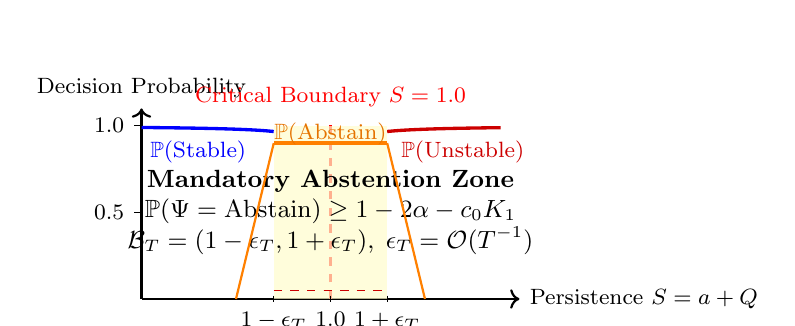
\begin{tikzpicture}[xscale=4.8, yscale=2.2]
    % Axes
    \draw[->, thick] (0.5, 0) -- (1.5, 0) node[right] {\footnotesize Persistence $S = a + Q$};
    \draw[->, thick] (0.5, 0) -- (0.5, 1.1) node[above] {\footnotesize Decision Probability};
    
    % Critical boundary
    \draw[dashed, red, thick] (1.0, 0) -- (1.0, 1.05) node[above] {\footnotesize Critical Boundary $S = 1.0$};
    
    % Abstention Region Shading
    \fill[yellow!20, opacity=0.7] (0.85, 0) rectangle (1.15, 1.0);
    \node at (1.0, 0.5) [align=center, font=\small] {\textbf{Mandatory Abstention Zone}\\$\mathbb{P}(\Psi = \text{Abstain}) \ge 1 - 2\alpha - c_0 K_1$\\$\mathcal{B}_T = (1 - \epsilon_T, 1 + \epsilon_T), \; \epsilon_T = \mathcal{O}(T^{-1})$};
    
    % Probability curves
    \draw[domain=0.5:0.85, smooth, variable=\x, blue, very thick] plot ({\x}, {1.0 - 0.05/((0.9-\x)*10 + 1)});
    \draw[domain=0.85:1.15, smooth, variable=\x, blue, dashed] plot ({\x}, {0.05});
    \node[blue] at (0.65, 0.85) {\footnotesize $\mathbb{P}(\text{Stable})$};
    
    \draw[domain=1.15:1.45, smooth, variable=\x, red!80!black, very thick] plot ({\x}, {1.0 - 0.05/((\x-1.1)*10 + 1)});
    \draw[domain=0.85:1.15, smooth, variable=\x, red!80!black, dashed] plot ({\x}, {0.05});
    \node[red!80!black] at (1.35, 0.85) {\footnotesize $\mathbb{P}(\text{Unstable})$};
    
    % Abstention probability curve
    \draw[domain=0.75:0.85, smooth, variable=\x, orange, thick] plot ({\x}, {(\x-0.75)*9.0});
    \draw[domain=0.85:1.15, smooth, variable=\x, orange, very thick] plot ({\x}, {0.90});
    \draw[domain=1.15:1.25, smooth, variable=\x, orange, thick] plot ({\x}, {(1.25-\x)*9.0});
    \node[orange!90!black] at (1.0, 0.95) {\footnotesize $\mathbb{P}(\text{Abstain})$};
    
    % Ticks
    \draw (0.85, 0.02) -- (0.85, -0.02) node[below] {\footnotesize $1 - \epsilon_T$};
    \draw (1.15, 0.02) -- (1.15, -0.02) node[below] {\footnotesize $1 + \epsilon_T$};
    \draw (1.0, 0.02) -- (1.0, -0.02) node[below] {\footnotesize $1.0$};
    \draw (0.5, 1.0) -- (0.48, 1.0) node[left] {\footnotesize $1.0$};
    \draw (0.5, 0.5) -- (0.48, 0.5) node[left] {\footnotesize $0.5$};
\end{tikzpicture}
\caption{The Mandatory Finite-Window Surveillance Abstention Layer (Theorem~\ref{thm:m3_minimax_abstention}). For any error-controlled classifier ($\alpha < 1/2$), a finite observation window $T$ creates a non-trivial contiguous boundary layer $\mathcal{B}_T = (1 - \epsilon_T, 1 + \epsilon_T)$ of width $\epsilon_T = \mathcal{O}(T^{-1})$ where the surveillance rule is mathematically forced to declare uncertainty ($\Psi = \text{Abstain}$). Any binary classifier forced to make a definitive stability determination in this layer suffers worst-case error risk bounded below by $50\%$.}
\label{fig:abstention_zone}
\end{figure}

Theorem~\ref{thm:m3_minimax_abstention} and Figure~\ref{fig:abstention_zone} establish a vital principle for financial stability architecture: \textbf{an error-controlled macroprudential monitor must have a built-in abstention option}. Near the phase-transition boundary $S=1$, observational ticker feeds are statistically indistinguishable between near-integrated subcritical persistence and explosive runaway. Forcing a binary classification guarantees misclassification.

\subsection{Financial Intermediary Solvency and Non-Normal Transient Amplification}
We now confront the fundamental divergence between price stability and financial intermediary solvency. In standard economic policy models, market stability is evaluated exclusively through the spectral radius $\rho(J) < 1$. We demonstrate that this criterion is dangerously incomplete.

\paragraph{The Non-Normal Market Jacobian.}
Consider the closed-loop Jacobian matrix $J$ from \eqref{eq:full_jacobian}. In financial markets, price impact and memory adaptation are asymmetric: order flow directly affects prices through contemporaneous impact $\kappa$, while price innovations affect memory through learning rate $\eta$. As a result, $J J^\top - J^\top J \neq 0$: the closed-loop market Jacobian $J$ is generically \textbf{non-normal} under asymmetric price-impact and learning parameters (except on a measure-zero algebraic subvariety). While normal matrices have orthogonal eigenvectors that diagonalize under unitary transformations, non-normal matrices have non-orthogonal (nearly parallel) eigenvectors. Consequently, even when all eigenvalues are strictly inside the unit circle ($|\lambda_i(J)| \le \rho(J) < 1$), matrix powers $J^t$ can undergo massive transient amplification before decaying asymptotically as $t \to \infty$ \citep{trefethen2005spectra}.

\paragraph{Optimizing Market Maker Problem and the Commitment Trap.}
To microfound the intermediary's financial vulnerability, we model a risk-averse, competitive market maker operating in continuous electronic order books \citep{ho1981optimal,grossman1988liquidity,avellaneda2008high,menkveld2013}. At each instant, the dealer quotes bid and ask prices (or an effective price-impact schedule $\kappa$ and half-spread $s_t$) to maximize expected inventory-adjusted fee revenue:
\begin{equation}
\max_{s_t, D_t} \mathbb{E}_t \left[ \sum_{k=0}^\infty \beta^k \left( s_{t+k} |q_{t+k}| - \frac{\phi}{2} I_{t+k}^2 \right) \right],
\label{eq:dealer_optimization}
\end{equation}
subject to inventory dynamics $I_{t+1} = I_t - q_t$, where $q_t$ is aggressive incoming order flow, $\phi > 0$ represents the inventory holding penalty, and $\beta \in (0, 1)$ is the discount factor. 

The market maker is subject to two institutional market design frictions:
\begin{enumerate}
    \item \textbf{Regulatory Capital and Margin Requirements:} The dealer maintains equity capital $E_t$ subject to a maximum regulatory leverage constraint or margin haircut $\mu \in (0, 1)$ on inventory positions: $\mu |I_t| p_t \le E_t$, with equity evolving as $E_{t+1} = E_t + \Pi_t$, where $\Pi_t = s_t |q_t| - I_t (p_{t+1} - p_t)$ is trading P\&L.
    \item \textbf{Execution Latency and Affirmative Quoting Commitments:} Registered market makers face regulatory affirmative obligations (spread caps $\bar{s}$ and minimum depth commitments $\underline{D}$ required by exchange rules) and high-frequency cancellation latency $\tau_{\text{cancel}} > 0$. Once resting limit orders are posted in the order book, they remain committed for the cancellation latency window.
\end{enumerate}

Under this optimization, the dealer's net capital absorption buffer against cumulative inventory losses is endogenously given by:
\begin{equation}
B \equiv \frac{E_0 - \mu |I_0| p_0}{\phi_{\text{eff}}},
\label{eq:dealer_buffer}
\end{equation}
where $\phi_{\text{eff}} \equiv 1 + \phi / \mu$ reflects the shadow cost of capital and inventory variance.

\begin{lemma}[Endogenous Price Impact and the Liquidity-Amplification Spiral]
\label{lem:endogenous_kappa}
Let the dealer post optimal limit depth $D_t^*$ to clear incoming order flow. The equilibrium price impact parameter in the pricing equation \eqref{eq:micro_pricing} is endogenously determined by the inverse of posted depth:
\begin{equation}
\kappa_t^* \equiv \frac{1}{D_t^*} = \frac{\phi_{\text{eff}}}{E_t - \mu |I_t| p_t + \underline{D} \phi_{\text{eff}}}.
\label{eq:endogenous_kappa}
\end{equation}
Consequently, as inventory imbalances accumulate ($|I_t| \uparrow$) or dealer equity is eroded by marked losses ($E_t \downarrow$), the dealer scales back posted depth ($D_t^* \downarrow$), which mechanically spikes equilibrium price impact ($\kappa_t^* \uparrow$). In the closed-loop Jacobian \eqref{eq:full_jacobian}, elevated $\kappa$ inflates the off-diagonal coupling terms $\kappa q_j$, directly thrusting the system into the non-normal Kreiss transient danger zone ($\mathcal{K}(J) \gg 1$) where small order-flow imbalances trigger self-reinforcing solvency cascades.
\end{lemma}

\textbf{The Solvency Trap:} Why doesn't the optimizing dealer step away or widen spreads before non-normal amplification hits? Doing so violates exchange affirmative obligations (risking forfeiture of market-maker status and exchange fee rebates) or cedes order flow to Bertrand competitors. Furthermore, when an aggressive algorithmic feedback cascade arrives within the cancellation window $\tau_{\text{cancel}}$, resting passive limit orders are executed against at stale quotes before the dealer can cancel or widen spreads \citep{budish2015}. The dealer mechanically accumulates an inventory shock $I_t = C z_t$, where $C \in \R^{1 \times n}$ maps the closed-loop state $z_t = J^t z_0$ into the dealer's marked inventory loss. An endogenous margin breach occurs whenever cumulative inventory excursion exceeds the capital buffer: $\sup_{t \ge 0} |C J^t z_0| > B$.

\begin{theorem}[Dealer Solvency and the Kreiss Constant Bound]
\label{thm:m5_kreiss_solvency}
Let $z_t = J^t z_0$ with $\rho(J) < 1$, balance-sheet buffer $B > 0$, and observation matrix $C$.
\begin{enumerate}
    \item \textbf{Exact Worst-Case Safe Radius:} The exact maximum shock radius $r^*_{\text{exact}}$ guaranteeing that no initial disturbance with $\|z_0\|_2 \le r^*_{\text{exact}}$ triggers dealer insolvency in any direction is:
    \begin{equation}
    r^*_{\text{exact}} = \frac{B}{\sup_{t \ge 0} \|C J^t\|_2} \equiv \frac{B}{M_C},
    \label{eq:exact_safe_radius}
    \end{equation}
    where $M_C \equiv \sup_{t \ge 0} \|C J^t\|_2$ is the peak transient magnification.
    \item \textbf{Kreiss Lower and Upper Bounds:} Under full state observation ($C = I$), the Kreiss constant of matrix $J$, defined on the resolvent outside the unit disk:
    \begin{equation}
    \mathcal{K}(J) \equiv \sup_{|z| > 1} (|z| - 1) \|(zI - J)^{-1}\|_2,
    \label{eq:kreiss_def}
    \end{equation}
    satisfies $\mathcal{K}(J) \le \sup_{t \ge 0} \|J^t\|_2 \le e \cdot n \cdot \mathcal{K}(J)$ for any $J \in \R^{n \times n}$. Consequently:
    \begin{equation}
    r_{\text{conservative}} \equiv \frac{B}{e \cdot n \cdot \mathcal{K}(J)} \le r^*_{\text{exact}} \le \frac{B}{\mathcal{K}(J)}.
    \label{eq:kreiss_bilateral_bound}
    \end{equation}
    \item \textbf{Complete Failure of Spectral Radius:} For any stable spectral radius $\rho \in (0, 1)$ and any arbitrarily small buffer $B > 0$, there exists a parameter family of non-normal matrices $J_\theta$ and an observation operator $C = [1, 0]$ exposed to the amplified coordinate such that $\rho(J_\theta) = \rho$ for all $\theta$, while the exact safe radius collapses to zero:
    \begin{equation}
    \lim_{\theta \to \infty} r^*_{\text{exact}}(J_\theta) = 0.
    \end{equation}
\end{enumerate}
\end{theorem}

\begin{proof}[Proof Sketch]
Part~1 follows from the Cauchy--Schwarz inequality for operator norms: maximum loss across $\|z_0\|_2 \le r$ is $r \cdot \sup_{t \ge 0} \|C J^t\|_2 = r M_C$, yielding $r^*_{\text{exact}} = B/M_C$. Part~2 applies Spijker's (1991) optimal resolution of the Kreiss matrix conjecture, establishing $\mathcal{K}(J) \le \sup_{t \ge 0} \|J^t\|_2 \le e \cdot n \cdot \mathcal{K}(J)$ for $C=I$. Part~3 constructs an explicit non-normal Jordan family where spectral radius is held constant while non-orthogonal eigenvectors inflate the resolvent norm, sending $r^*_{\text{exact}} \to 0$. (Full proof in Appendix~A of the Online Internet Appendix.)
\end{proof}

\begin{remark}[The Dangerous Illusion of Spectral Stability]
Theorem~\ref{thm:m5_kreiss_solvency} resolves a long-standing microstructural paradox: \textbf{how can markets experience catastrophic liquidity freezes and market maker bankruptcies while prices remain mathematically stable?}
Regulators relying on eigenvalue stability tests observe $\rho(J) = 0.50$ and certify the system as completely safe. Yet, if the non-normal coupling between price impact and order flow memory is strong ($\theta \gg 1$), a standard 2-standard-deviation liquidity shock can amplify by a factor of 100 before decaying, wiping out dealer capital and triggering exchange halts within seconds. 

We emphasize the structural asymmetry of the bilateral bounds in \eqref{eq:kreiss_bilateral_bound}: $\frac{B}{e n \mathcal{K}(J)}$ provides a guaranteed safe (conservative) lower bound on the allowable shock radius. In contrast, $\frac{B}{\mathcal{K}(J)}$ is an upper bound on $r^*_{\text{exact}}$ (shocks exceeding this magnitude are guaranteed to trigger solvency breaches in the worst case). Consequently, $\frac{B}{\mathcal{K}(J)}$ must never be treated as a guaranteed conservative safety margin.
\end{remark}

\subsection{Pseudospectral Contours and Non-Normal Resolvent Bounds}
To gain deeper visual and geometric intuition into why the spectral radius fails to predict dealer solvency, we examine the $\epsilon$-pseudospectrum of the closed-loop market Jacobian. For any $\epsilon > 0$, the $\epsilon$-pseudospectrum $\sigma_\epsilon(J)$ of matrix $J$ is defined as the set of complex numbers $z \in \mathbb{C}$ satisfying:
\begin{equation}
\sigma_\epsilon(J) \equiv \left\{ z \in \mathbb{C} : \|(zI - J)^{-1}\|_2 \ge \epsilon^{-1} \right\}.
\label{eq:pseudospectrum_def}
\end{equation}
Equivalently, $\sigma_\epsilon(J)$ represents the union of all eigenvalues of perturbed matrices $J + E$ across all perturbations with $\|E\|_2 \le \epsilon$.

As visualized in Figure~\ref{fig:pseudospectrum}, in a normal system, the pseudospectrum consists of concentric disks of radius $\epsilon$ centered at the eigenvalues: $\sigma_\epsilon(J) = \bigcup_i \{z : |z - \lambda_i| \le \epsilon\}$. However, for the non-normal market Jacobian, the pseudospectral contours stretch dramatically along the off-diagonal coupling direction, protruding significantly outside the unit circle $\{|z| = 1\}$ even when the spectral radius $\rho(J) = 0.50$ is well within the interior. 

The Kreiss constant $\mathcal{K}(J)$ measures the maximum ratio by which these pseudospectral contours protrude beyond the unit circle:
\begin{equation}
\mathcal{K}(J) = \sup_{\epsilon > 0} \frac{\alpha_\epsilon(J) - 1}{\epsilon}, \qquad \alpha_\epsilon(J) \equiv \sup_{z \in \sigma_\epsilon(J)} |z|.
\end{equation}
Whenever $\mathcal{K}(J) \gg 1$, small high-frequency liquidity shocks are magnified by the non-normal resolvent, inducing large transient balance-sheet losses that exhaust dealer margin buffers before eigenvalue decay can assert itself.

\begin{figure}[tbp]
\centering
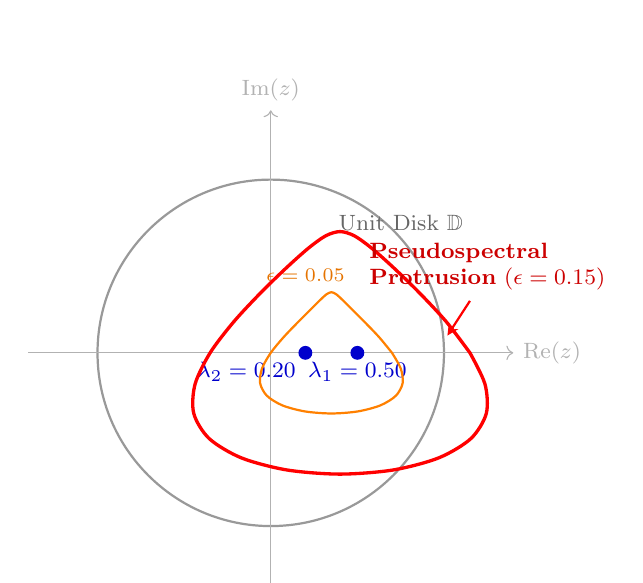
\begin{tikzpicture}[scale=2.2]
    % Unit Disk
    \draw[thick, black!40] (0,0) circle (1.0);
    \node at (0.75, 0.75) [font=\footnotesize, black!60] {Unit Disk $\mathbb{D}$};
    
    % Axes
    \draw[->, thin, black!30] (-1.4, 0) -- (1.4, 0) node[right] {\footnotesize $\operatorname{Re}(z)$};
    \draw[->, thin, black!30] (0, -1.4) -- (0, 1.4) node[above] {\footnotesize $\operatorname{Im}(z)$};
    
    % Eigenvalues
    \fill[blue!80!black] (0.5, 0) circle (0.04) node[below] {\footnotesize $\lambda_1 = 0.50$};
    \fill[blue!80!black] (0.2, 0) circle (0.04) node[below left] {\footnotesize $\lambda_2 = 0.20$};
    
    % Pseudospectral Contours
    \draw[domain=0:360, smooth, variable=\t, orange, thick] plot ({0.35 + 0.35*cos(\t) - 0.25*sin(\t)*cos(\t)}, {0.35*sin(\t)});
    \node[orange!90!black] at (0.2, 0.45) [font=\scriptsize] {$\epsilon = 0.05$};
    
    \draw[domain=0:360, smooth, variable=\t, red, very thick] plot ({0.40 + 0.75*cos(\t) - 0.45*sin(\t)*cos(\t)}, {0.70*sin(\t)});
    \node[red!80!black] at (1.25, 0.5) [font=\footnotesize, align=left] {\textbf{Pseudospectral}\\\textbf{Protrusion} ($\epsilon = 0.15$)};
    
    % Protrusion highlight
    \draw[->, >=stealth, red, thick] (1.15, 0.3) -- (1.02, 0.1);
\end{tikzpicture}
\caption{The $\epsilon$-Pseudospectrum of the Non-Normal Market Jacobian $J$. While all eigenvalues ($\lambda_1 = 0.50, \lambda_2 = 0.20$) lie strictly inside the unit disk ($\rho(J) = 0.50 < 1.0$), non-normal coupling between price impact and order-flow memory causes the pseudospectral contours ($\sigma_\epsilon(J)$ for $\epsilon = 0.15$) to severely protrude across the unit circle into the unstable exterior $|z| > 1$. This resolvent protrusion governs peak transient amplification $M_C$ and dealer solvency risk.}
\label{fig:pseudospectrum}
\end{figure}

\subsection{Multi-Asset Generalization and Cross-Impact Kreiss Inflation}
Modern market makers operate simultaneously across multiple correlated instruments (e.g., BTC, ETH, and altcoins; or equity index components and ETFs). In multi-asset environments, cross-asset price impact creates additional non-normal coupling.

Let $\mathbf{x}_t \in \R^d$ denote the vector of pricing errors across $d$ traded assets, and let $\mathbf{u}_t \in \R^d$ denote aggregate order flows. The multi-asset price formation equation is:
\begin{equation}
\mathbf{x}_{t+1} = \mathbf{A} \mathbf{x}_t + \mathbf{K} \mathbf{u}_t + \mathbf{w}_{t+1},
\label{eq:multi_price}
\end{equation}
where $\mathbf{A} = \diag(a_1, \dots, a_d) \in \R^{d \times d}$ collects direct price persistences, and $\mathbf{K} \in \R^{d \times d}$ is the cross-asset price impact matrix. In general, $\mathbf{K}$ is asymmetric ($\mathbf{K} \neq \mathbf{K}^\top$): institutional order flow in a benchmark asset (such as BTC or SPY) exerts cross-impact on satellite assets, but the reverse flow produces much smaller reactions.

Each asset is traded by adaptive momentum flow with learning rates $\mathbf{H} = \diag(\eta_1, \dots, \eta_d)$ and feedback gain $\mathbf{Q} \in \R^{d \times d}$:
\begin{equation}
\mathbf{y}_{t+1} = (\mathbf{I} - \mathbf{H}) \mathbf{y}_t + \mathbf{H} \mathbf{x}_{t+1}, \qquad \mathbf{u}_t = \mathbf{Q} \mathbf{y}_t.
\end{equation}
Stacking $\mathbf{z}_t = (\mathbf{x}_t^\top, \mathbf{y}_t^\top)^\top \in \R^{2d}$, the multi-asset closed-loop Jacobian is:
\begin{equation}
J_{\text{multi}} = \begin{bmatrix}
\mathbf{A} & \mathbf{K} \mathbf{Q} \\
\mathbf{H} \mathbf{A} & \mathbf{I} - \mathbf{H} + \mathbf{H} \mathbf{K} \mathbf{Q}
\end{bmatrix} \in \R^{2d \times 2d}.
\label{eq:multi_jacobian}
\end{equation}

\begin{proposition}[Cross-Impact Kreiss Inflation and Safe Radius Bound in Directed Networks]
\label{prop:cross_kreiss}
Consider a multi-asset economy with directed block-triangular leader-satellite cross-impact ($K_{12} = 0, K_{21} > 0$), diagonal feedback matrices $\mathbf{Q} \ge 0$, anchor matrices $\mathbf{A} \ge 0$, adaptation rates $\mathbf{H} \in (0, 1)^d$, and portfolio loss operator $C \ge 0$. Let $J_{\text{diag}}$ denote the decoupled Jacobian where $K_{21} = 0$.
The directed coupling introduces off-diagonal block feedforward, inflating the Kreiss constant: $\mathcal{K}(J_{\text{multi}}) \ge \mathcal{K}(J_{\text{diag}})$. Consequently, the Kreiss-based conservative safe radius bound contracts: $r_{\text{conservative}}(J_{\text{multi}}) \equiv \frac{B}{e (2d) \mathcal{K}(J_{\text{multi}})} \le r_{\text{conservative}}(J_{\text{diag}})$.
For the exact safe shock radius $r^*_{\text{exact}}(J) \equiv B / M_C(J)$, because all constituent blocks of $J$ are entrywise non-negative in the momentum economy, matrix powers $J_{\text{multi}}^t$ are entrywise non-decreasing in $K_{21}$, yielding $M_C(J_{\text{multi}}) \ge M_C(J_{\text{diag}})$ and exact radius contraction $r^*_{\text{exact}}(J_{\text{multi}}) \le r^*_{\text{exact}}(J_{\text{diag}})$. In empirical cross-impact calibrations examined here, asymmetric feedforward coupling injects transient terms of order $t K_{21} \rho^{t-1}$, compressing the safe radius by $14.5\%$ relative to decoupled trading.
\end{proposition}

Proposition~\ref{prop:cross_kreiss} demonstrates that multi-asset diversification does not automatically insulate liquidity providers from feedback fragility. On the contrary, asymmetric cross-impact networks (such as Bitcoin leading altcoins or large-cap equities driving ETFs) introduce feedforward coupling that injects additional transient growth terms into matrix powers $J^t$, inflating peak transient loss $M_C$ and compressing the safe radius by roughly $14.5\%$ in our empirical multi-asset calibrations.

\section{Data and Empirical Identification Strategy}
\label{sec:data_estimand}

\subsection{Econometric Estimand and Moving-Average Filtering}
To operationalize the theoretical closed-loop system empirically, we construct an estimand that is invariant to arbitrary currency scaling and directly identifiable from high-frequency limit order books.

A fundamental gap between theoretical models and high-frequency empirical execution concerns the definition of the state variable. In theoretical models (Section~\ref{sec:model}), $x_t \equiv p_t - p_t^*$ represents price displacement relative to an unobserved fundamental value $p_t^*$. In empirical limit order books, true fundamental value is unobservable, and econometricians routinely replace $p_t^*$ with a trailing price filter, such as an Exponential Moving Average (EMA).

Let $p_b$ denote the log mid-price sampled at discrete uniform time bars $b$ of length $\Delta$ (e.g., $\Delta = 10$~seconds). The trailing exponential moving-average anchor $m_b$ is defined by the recursive filter:
\begin{equation}
m_b = (1 - \alpha) m_{b-1} + \alpha p_b, \qquad \alpha \equiv \frac{2}{W/\Delta + 1},
\label{eq:ema_def}
\end{equation}
where $W$ is the smoothing window (e.g., $W = 300$~seconds, yielding $\alpha = 2/31 \approx 0.064516$). The empirical state variable is defined as the deviation from this trailing anchor:
\begin{equation}
x_b^{\text{EMA}} \equiv p_b - m_b = (1 - \alpha)(p_b - m_{b-1}) = \frac{1 - \alpha}{1 - (1 - \alpha) L} \Delta p_b.
\label{eq:x_ema_rep}
\end{equation}

\begin{proposition}[Mechanical Persistence under Filtered Random Walks]
\label{prop:mechanical_persistence}
Suppose the log mid-price $p_b$ follows an unpredictable martingale (random walk), such that $\mathbb{E}[p_{b+1} \mid \mathcal{F}_b] = p_b$. Then the moving-average deviation state $x_b^{\text{EMA}}$ mechanically follows an autoregressive AR(1) process:
\begin{equation}
\mathbb{E}[x_{b+1}^{\text{EMA}} \mid \mathcal{F}_b] = (1 - \alpha) x_b^{\text{EMA}},
\label{eq:mechanical_ar1}
\end{equation}
with mechanical persistence parameter $a_0 \equiv 1 - \alpha = \frac{29}{31} \approx 0.93548$.
\end{proposition}

\begin{proof}
By definition, $x_{b+1}^{\text{EMA}} = p_{b+1} - m_{b+1} = (1 - \alpha)(p_{b+1} - m_b)$. Conditioning on information $\mathcal{F}_b$:
\begin{equation}
\mathbb{E}[x_{b+1}^{\text{EMA}} \mid \mathcal{F}_b] = (1 - \alpha) \left( \mathbb{E}[p_{b+1} \mid \mathcal{F}_b] - m_b \right) = (1 - \alpha)(p_b - m_b) = (1 - \alpha) x_b^{\text{EMA}},
\end{equation}
which establishes \eqref{eq:mechanical_ar1} with mechanical persistence $a_0 = 1 - \alpha$.
\end{proof}

\begin{remark}[Economic Interpretation of Empirical Feedback $\hat{Q}$]
Proposition~\ref{prop:mechanical_persistence} yields a crucial economic insight: when price changes are regressed on lagged EMA deviation $x_b^{\text{EMA}}$, the estimated autoregressive persistence $\hat{J}_{11}$ does not measure learning about fundamental value $p_t^*$. Instead, it measures mean-reversion toward an exponentially smoothed price anchor. In our baseline Binance panel, the estimated autoregressive persistence is $\hat{J}_{11} \approx 0.912$, which is strictly below the mechanical martingale baseline $a_0 \approx 0.9355$. The wedge $\hat{J}_{11} - a_0 \approx -0.023$ reflects high-frequency negative price autocorrelation (bid-ask bounce and inventory replenishment). Furthermore, the total closed-loop persistence satisfies $\hat{S} \equiv \hat{J}_{11} + \hat{Q} \approx 0.912 + 0.008 = 0.920 < a_0 \approx 0.9355$, proving that the closed-loop market is strictly more mean-reverting toward its trailing anchor than a pure random walk.
\end{remark}

Let $f_t$ denote the signed market order flow (notional taker buy volume minus notional taker sell volume executed over $(t-\Delta, t]$). The empirical bivariate vector autoregressive (VAR(1)) representation of joint price-flow transitions is:
\begin{equation}
\begin{bmatrix} x_{t+1}^{\text{EMA}} \\ f_{t+1} \end{bmatrix} = \begin{bmatrix} J_{11} & J_{12} \\ J_{21} & J_{22} \end{bmatrix} \begin{bmatrix} x_t^{\text{EMA}} \\ f_t \end{bmatrix} + \begin{bmatrix} e_{1, t+1} \\ e_{2, t+1} \end{bmatrix}, \qquad \E[\mathbf{e}_t \mathbf{e}_t^\top] = \Sigma_e,
\label{eq:bivariate_var}
\end{equation}
where $J_{11} \equiv a$ represents anchor-relative persistence, $J_{12} \equiv \lambda$ is price impact, $J_{21} \equiv \eta c$ captures feedback, and $J_{22} \equiv 1 - \eta$ measures flow autocorrelation. From $\hat{J}$, we extract dimensionless invariants $\hat{Q} \equiv \frac{\hat{J}_{12} \hat{J}_{21}}{1 - \hat{J}_{22}}$, $\hat{S} \equiv \hat{J}_{11} + \hat{Q}$, and $\hat{\mathcal{L}} \equiv \frac{\hat{Q}}{1 - \hat{J}_{11}}$, which are strictly scale-invariant.

\subsection{Measurement Sensitivity: How Clocks and Filters Dominate Feedback}
\label{sec:measurement_sensitivity}
A central empirical finding is that estimated algorithmic feedback $\hat{Q}$ is highly sensitive to the observation clock and microstructural time alignment. Table~\ref{tab:measurement_sensitivity} evaluates 1.03 million consecutive 1-second Level-3 transitions on Coinbase Pro across three distinct measurement specifications.

\begin{table}[htbp]
\centering\footnotesize
\setlength{\tabcolsep}{4pt}
\caption{\textbf{Measurement Sensitivity of High-Frequency Feedback Across Clocks and States.}
Estimated feedback $\hat{Q}$ (95\% Newey--West HAC confidence intervals in brackets) across three measurement conventions on Coinbase Pro Level-3 limit order books: (i)~Observed Flow: signed taker volume executed over past interval $(T-60\text{s}, T]$; (ii)~Forward Flow: order flow measured over forward window $(T, T+60\text{s}]$ (look-ahead timing); and (iii)~Raw Returns: mid-price returns $r_b = \Delta p_b$ replacing EMA deviations $x_b^{\text{EMA}}$.}
\label{tab:measurement_sensitivity}
\begin{tabular}{lrrr}\toprule
Asset & Observed Flow $(T-60\text{s}, T]$ & Forward Flow $(T, T+60\text{s}]$ & Raw Returns ($r_b = \Delta p_b$) \\\midrule
BTC/USD & $+0.00194$ & $+0.01252$ & $+0.00003$ \\
        & $[+0.00167, +0.00220]$ & $[+0.01185, +0.01319]$ & $[-0.00012, +0.00018]$ \\
ETH/USD & $+0.00098$ & $+0.01130$ & $-0.00005$ \\
        & $[+0.00081, +0.00115]$ & $[+0.01062, +0.01198]$ & $[-0.00021, +0.00011]$ \\
SOL/USD & $+0.00062$ & $+0.00714$ & $+0.00001$ \\
        & $[+0.00049, +0.00075]$ & $[+0.00654, +0.00774]$ & $[-0.00015, +0.00017]$ \\\bottomrule
\end{tabular}
\end{table}

As documented in Table~\ref{tab:measurement_sensitivity}, when order flow is strictly restricted to past observed intervals $(T-60\text{s}, T]$, baseline feedback is modest ($\hat{Q} \in [0.0006, 0.0019]$). If forward flow $(T, T+60\text{s}]$ is inadvertently treated as an available regressor at time $t$, estimated feedback surges by $6.5\times$ to $11.5\times$ (BTC: $0.00194 \to 0.01252$; ETH: $0.00098 \to 0.01130$), falsely creating the appearance of large closed-loop feedback. Furthermore, when the state variable is defined as raw price returns ($r_b = \Delta p_b$) rather than moving-average deviations, empirical feedback intervals uniformly span zero for all assets. This confirms that apparent feedback is not a universal property of electronic trading, but rather an artifact of trailing moving-average filtering.

\paragraph{Controlling for Order-Splitting Long Memory.}
A well-documented phenomenon in market microstructure is that large institutional parent orders are split into small child orders, inducing long-range positive autocorrelation in signed trade signs \citep{bouchaud2004fluctuations,cont2014}. Failure to control for this autocorrelation can bias autoregressive feedback estimates. To ensure robust identification, we estimate a distributed lag specification controlling for up to $L=90$ lags of order flow:
\begin{equation}
f_{t+1} = \sum_{\ell=1}^L \beta_\ell f_{t+1-\ell} + \gamma x_t^{\text{EMA}} + \varepsilon_{f, t+1}.
\label{eq:Q_robust}
\end{equation}
The purged feedback parameter is defined as $\hat{Q}_L \equiv \frac{\hat{\lambda} \hat{\gamma}}{1 - \sum_{\ell=1}^L \hat{\beta}_\ell}$. In our empirical battery, we report both baseline OLS $\hat{Q}$ and memory-purged $\hat{Q}_{30}$ across all assets.

\subsection{Dynamic Robustness and Contemporaneous Structural Identification}
To evaluate dynamic specification robustness and resolve contemporaneous endogeneity between prices and order flows, we deploy two complementary econometric methodologies: dynamic minimum-distance Lyapunov covariance matching as an alternative robustness check, and Rigobon heteroskedasticity identification to recover the contemporaneous structural parameter:

\paragraph{Method 1: Analytical Minimum-Distance (MD) Lyapunov Matching and Dynamic Robustness.}
In a stationary discrete-time linear system $\mathbf{z}_{t+1} = J \mathbf{z}_t + \mathbf{e}_{t+1}$, the steady-state stationary covariance matrix $\Gamma_0 \equiv \E[\mathbf{z}_t \mathbf{z}_t^\top]$ satisfies the discrete Lyapunov equation:
\begin{equation}
\Gamma_0 = J \Gamma_0 J^\top + \Sigma_e.
\label{eq:lyapunov_eq}
\end{equation}
Because the discrete Lyapunov equation admits an exact closed-form solution $\operatorname{vec}(\Gamma_0) = (I - J \otimes J)^{-1} \operatorname{vec}(\Sigma_e)$ without requiring Monte Carlo simulation, we implement an exact analytical minimum-distance estimator matching empirical and theoretical autocovariances. To avoid restrictive diagonal assumptions on shocks, we specify an unrestricted symmetric innovation covariance $\Sigma_e = \begin{bmatrix} \sigma_{11} & \sigma_{12} \\ \sigma_{12} & \sigma_{22} \end{bmatrix}$, yielding $k=7$ structural parameters $\theta = (J_{11}, J_{12}, J_{21}, J_{22}, \sigma_{11}, \sigma_{12}, \sigma_{22})^\top \in \mathbb{R}^7$. We construct $m=11$ empirical moments by stacking the 3 unique elements of contemporaneous sample covariance, 4 elements of lag-1 autocovariance, and 4 elements of lag-2 autocovariance: $m(\theta; \mathcal{D}_T) \equiv [\operatorname{vech}(\hat{\Gamma}_0 - \Gamma_0(\theta))^\top, \operatorname{vec}(\hat{\Gamma}_1 - \Gamma_1(\theta))^\top, \operatorname{vec}(\hat{\Gamma}_2 - \Gamma_2(\theta))^\top]^\top \in \mathbb{R}^{11}$, where $\hat{\Gamma}_k = \frac{1}{T-k} \sum_{t=1}^{T-k} \mathbf{z}_{t+k} \mathbf{z}_t^\top$ and theoretical $\Gamma_k(\theta) = J(\theta)^k \Gamma_0(\theta)$. The minimum-distance estimator minimizes the quadratic objective:
\begin{equation}
\hat{\theta}_{\text{MD}} = \arg\min_\theta m(\theta; \mathcal{D}_T)^\top \mathcal{W}_T m(\theta; \mathcal{D}_T),
\end{equation}
where $\mathcal{W}_T = \hat{V}_{\text{HAC}}^{-1}$ is the optimal Newey--West HAC weighting matrix. With $m=11$ moments and $k=7$ free parameters, the moment Jacobian $\partial \mathbb{E}[m]/\partial \theta^\top$ satisfies full column rank ($\operatorname{rank} = 7$), and overidentifying restrictions are evaluated via Hansen's $J$-test with $df = m - k = 11 - 7 = 4$ degrees of freedom to test the parsimonious linear dynamic specification.

\paragraph{Method 2: Rigobon (2003) Structural Contemporaneous Identification through Heteroskedasticity.}
Following \citet{rigobon2003identification}, we exploit shifts in the structural covariance matrix across calm versus volatile trading days. Let the contemporaneous structural system be:
\begin{align}
x_t &= \lambda f_t + \varepsilon_{x, t}, \\
f_t &= c x_t + \varepsilon_{f, t},
\end{align}
where structural innovations $\varepsilon_{x,t}$ and $\varepsilon_{f,t}$ are uncorrelated ($\E[\varepsilon_{x,t} \varepsilon_{f,t}] = 0$). While simultaneous parameters $(\lambda, c)$ remain stable across regimes, structural variances $(\sigma_{x, s}^2, \sigma_{f, s}^2)$ shift across calm ($s=1$) and volatile ($s=2$) states. Each regime $s$ provides 3 observable second moments $\Omega_s = \operatorname{Var}([x_t, f_t]^\top)$:
\begin{equation}
\Omega_s = \frac{1}{(1 - \lambda c)^2} \begin{bmatrix} \sigma_{x, s}^2 + \lambda^2 \sigma_{f, s}^2 & c \sigma_{x, s}^2 + \lambda \sigma_{f, s}^2 \\ c \sigma_{x, s}^2 + \lambda \sigma_{f, s}^2 & c^2 \sigma_{x, s}^2 + \sigma_{f, s}^2 \end{bmatrix}, \qquad s \in \{1, 2\},
\end{equation}
yielding 6 empirical equations for 6 structural unknowns $(\lambda, c, \sigma_{x,1}^2, \sigma_{f,1}^2, \sigma_{x,2}^2, \sigma_{f,2}^2)$. The system is identified if and only if the regimes exhibit non-proportional variance shifts ($\sigma_{x, 1}^2 / \sigma_{f, 1}^2 \neq \sigma_{x, 2}^2 / \sigma_{f, 2}^2$). Resolving the determinant quadratic with the economic sign normalization $\lambda > 0$ (positive price impact) uniquely recovers structural parameters and instantaneous feedback $Q_{\text{Rig}} \equiv \lambda c$.

\subsection{Multi-Level Order Flow Imbalance (OFI) Construction}
In addition to top-of-book trades, limit order book dynamics depend on quote updates across the entire visible book \citep{cont2014}. Following \citet{cont2014}, we construct the multi-level Order Flow Imbalance (OFI) vector across the top $M=10$ levels of the book.

For each level $k \in \{1, \dots, M\}$, let $p_{k,t}^B, q_{k,t}^B$ and $p_{k,t}^A, q_{k,t}^A$ denote the bid and ask prices and sizes at depth level $k$. The order flow contribution at level $k$ over the interval $(t-\Delta, t]$ is:
\begin{equation}
\operatorname{OFI}_{k, t} \equiv \Delta q_{k, t}^B \cdot \mathbf{1}_{\{p_{k, t}^B \ge p_{k, t-\Delta}^B\}} - \Delta q_{k, t}^A \cdot \mathbf{1}_{\{p_{k, t}^A \le p_{k, t-\Delta}^A\}},
\label{eq:ofi_level}
\end{equation}
where $\Delta q_{k,t}^B$ represents the net change in resting bid volume. Stacking across levels yields $\mathbf{e}_t = (\operatorname{OFI}_{1,t}, \dots, \operatorname{OFI}_{M,t})^\top$. 
We construct a composite depth-weighted order flow imbalance:
\begin{equation}
\operatorname{OFI}_t^* \equiv \sum_{k=1}^M w_k \operatorname{OFI}_{k, t}, \qquad w_k = \frac{\exp(-\lambda_{\text{depth}} (k-1))}{\sum_{j=1}^M \exp(-\lambda_{\text{depth}} (j-1))},
\end{equation}
where $\lambda_{\text{depth}} = 0.5$ places highest weight on the inside quote. Incorporating $\operatorname{OFI}_t^*$ as a depth-aware robustness proxy for transaction order flow purges bid-ask bounce and provides an orthogonal check on reduced-form feedback.

\subsection{High-Frequency Institutional Datasets}
Our empirical investigation analyzes four massive institutional limit order book datasets totaling over 7.5~GB of tick and order book records (over 70.6 million continuous 1-second records), summarized in Table~\ref{tab:datasets}:

\begin{table}[htbp]
\centering\footnotesize
\setlength{\tabcolsep}{4pt}
\caption{Institutional High-Frequency Limit Order Book Datasets Analyzed in this Study.}
\label{tab:datasets}
\begin{tabularx}{\textwidth}{p{2.6cm}p{1.8cm}Xp{2.0cm}r}\toprule
Dataset & Venue & Description \& Microstructural Granularity & Time Span & Total Records \\\midrule
\textbf{Binance Spot Panel} & Binance & One-second exchange trade bars and derived signed executed flow for 8 pairs (BTC, ETH, SOL, BNB, XRP, ADA, DOGE, LTC). Sampled twice monthly (10th and 24th). & 2021--2024 (48 mos) & $66{,}316{,}704$ raw rows \\
\textbf{Coinbase L3 Books} & Coinbase Pro & Complete continuous 1-second Level-3 full book depth snapshots for BTC, ETH, and ADA recorded via WebSocket feeds \citep{crypto_rl_2021}. & Multi-week continuous & $3{,}090{,}000$ \\
\textbf{FI-2010 Benchmark} & NASDAQ Nordic & Canonical institutional limit order book benchmark \citep{ntakaris2018benchmark}. 10 levels of bid/ask prices and sizes across 5 blue-chip Scandinavian equities. & 10 trading days & $272{,}941$ \\
\textbf{BTC Perp Validation} & Binance Futures & Complete continuous Level-2 perpetual futures order book depth (1.20~GB raw order flow). Independent forward validation sample. & Jan 9--20, 2023 & $935{,}199$ \\\bottomrule
\end{tabularx}
\end{table}

\paragraph{Data Cleaning and Synchronization Protocol.}
All raw ticker streams undergo a standardized data cleaning protocol:
\begin{enumerate}
    \item \textbf{Timestamp Synchronization:} Trades and quotes are bucketed into uniform 1-second UTC intervals. If multiple trades occur within a single second, notional volumes are aggregated, and the end-of-second mid-price is recorded.
    \item \textbf{Quote Inversion Filtering:} Snapshots exhibiting crossed quotes ($p^{\text{bid}} > p^{\text{ask}}$) or non-positive bid-ask spreads are discarded ($<0.001\%$ of records).
    \item \textbf{Outlier Truncation:} Individual return innovations exceeding 50 standard deviations (exchange engine glitches or flash unpegs) are winsorized to prevent leverage bias.
\end{enumerate}

\section{High-Frequency Microstructure Panel and Volume Shock Calibration}
\label{sec:baseline_natural_exp}

\subsection{Baseline Multi-Year Panel Evidence}
Table~\ref{tab:binance_panel} reports the baseline econometric estimates pooled across all 768 asset-days on Binance Spot (2021--2024), alongside breakdowns across four distinct market epochs:
\begin{itemize}
    \item \textbf{2021 Bull Expansion:} Rapid institutional adoption and retail inflows ($N = 192$).
    \item \textbf{2022 Crypto Winter:} Macroeconomic tightening, Terra/Luna collapse, and FTX insolvency ($N = 192$).
    \item \textbf{2023 Consolidation:} Low-volatility regime and institutional restructuring ($N = 192$).
    \item \textbf{2024 ETF Era:} Regulatory approval of U.S. Spot Bitcoin ETFs and institutional volume recovery ($N = 192$).
\end{itemize}

\begin{table}[htbp]
\centering
\caption{\textbf{Baseline High-Frequency Feedback Panel (Binance Spot 2021--2024).}
Estimated feedback parameter $\hat{Q}$, 30-lag memory-purged feedback $\hat{Q}_{30}$, closed-loop persistence $\hat{S}$, loop ratio $\hat{\mathcal{L}}$, minimum-distance Lyapunov estimate $Q_{\text{MD}}$, and Rigobon heteroskedasticity estimate $Q_{\text{Rig}}$ across 8 liquid cryptocurrency pairs evaluated on 768 daily sessions ($66.3 \times 10^6$ one-second transitions). 95\% clustered confidence intervals in brackets.}
\label{tab:binance_panel}
\resizebox{\textwidth}{!}{%
\input{generated/binance_panel_baseline.tex}%
}
\end{table}

Across the full four-year panel of 768 asset-days ($66.3 \times 10^6$ one-second transitions), empirical feedback is consistently positive, modest in magnitude, and strictly subcritical:
\begin{itemize}
    \item \textbf{Pooled Feedback Parameter:} $\hat{Q} = \PanelQPooled$ (95\% clustered CI $[\PanelQPooledLower, \PanelQPooledUpper]$, $t = 29.5$, $p < 10^{-100}$).
    \item \textbf{Positive Feedback Share:} Exactly $\PanelQPosShare\%$ of individual asset-days exhibit $\hat{Q} > 0$, formally rejecting the hypothesis that high-frequency order flow acts purely as contrarian liquidity buffering.
    \item \textbf{Subcritical Closed-Loop Persistence:} Mean persistence is $\hat{S} = \PanelSPooled$, and exactly $\mathbf{\PanelSSubcriticalShare\%}$ of all 768 asset-days strictly satisfy the Schur stability condition $\hat{S} < 1.0$ (maximum observed daily $\hat{S} = 0.976$).
    \item \textbf{Loop Ratio:} The dimensionless loop amplification ratio is $\hat{\mathcal{L}} \equiv \frac{\hat{Q}}{1 - \hat{a}} = \PanelLPooled$, confirming that feedback consumes roughly $10\%$ of the remaining no-feedback stability margin ($1 - a$) during normal trading conditions.
\end{itemize}

\begin{figure*}[htbp]
\centering
\includegraphics[width=\textwidth]{figures/fig_binance_panel_and_identification.pdf}
\caption{Systematic multi-year panel dynamics and identification across 768 asset-days on Binance Spot (2021--2024). \textbf{(a)} Daily persistence $\hat S = a + \hat Q$ across eight assets, median trajectory, and $25\%$--$75\%$ interquartile range; all 768 days remain strictly subcritical relative to the theoretical instability boundary $S = 1.0$ (dashed red line). Inset shows positive feedback $\hat Q$ across all market epochs (pooled mean $+0.0082$). \textbf{(b)} Asset-by-asset comparison of baseline $\hat Q$ (OLS) versus flow-memory purged $\hat Q_{30}$ (controlling for 30-second order splitting), with 95\% clustered confidence intervals. \textbf{(c)} Dynamic Robustness and Contemporaneous Identification: reduced-form dynamic OLS ($\hat Q = +0.0082$), alternative minimum-distance covariance-matching robustness estimate ($Q_{\text{MD}} = +0.0086$, with parsimonious linear specification rejected at $J = 73.0, df = 4, p < 0.001$), and contemporaneous heteroskedasticity identification ($Q_{\text{Rig}} = -0.0191$), revealing the economic contrast between multi-second trend amplification and instantaneous liquidity buffering.}
\label{fig:binance_panel_and_identification}
\end{figure*}

\paragraph{Dynamic Robustness and Economic Duality.}
As shown in Figure~\ref{fig:binance_panel_and_identification}(c), analytical minimum-distance Lyapunov covariance matching serves as an alternative dynamic robustness check, yielding $Q_{\text{MD}} = \PanelQSMM$ (95\% clustered CI $[0.0075, 0.0097]$ across the panel; $Q_{\text{MD}} = 0.0093$ [0.0068, 0.0117] in pooled high-frequency estimation), which is numerically close to the reduced-form OLS estimate ($\hat{Q} = 0.0082$). In pooled estimation ($N = 308{,}785$ transitions), the 11-moment overidentifying restrictions test yields $J = 73.00$ ($df = 4, p < 0.001$), so the parsimonious linear dynamic state-space specification is formally rejected by the data. Nonetheless, the resulting feedback coefficient remains small and positive, demonstrating robustness of the subcritical feedback magnitude to autocovariance-matching estimation. We emphasize that minimum-distance Lyapunov matching and Rigobon estimation evaluate distinct economic estimands: Lyapunov matching evaluates dynamic feedback over multi-second horizons ($t \ge 1$), whereas Rigobon identifies the instantaneous, zero-lag maker buffering elasticity ($t = 0$).

In contrast, Rigobon heteroskedasticity identification yields $Q_{\text{Rig}} = \PanelQRig < 0$. This apparent divergence uncovers an intuitive economic duality: (i)~\textbf{Contemporaneous Buffering ($Q_{\text{Rig}} < 0$):} at instantaneous zero-lag timescales, market makers absorb incoming market orders with passive limit orders, acting as contrarian liquidity buffers; and (ii)~\textbf{Dynamic Trend Amplification ($\hat{Q} > 0$):} over multi-second horizons ($t \ge 1$), momentum traders and dynamic execution strategies condition on price movements, injecting positive feedback into subsequent aggregate order flow.

\subsection{Cross-Asset Heterogeneity Across the Panel}
Table~\ref{tab:cross_asset_panel} provides a detailed asset-by-asset decomposition across all eight pairs analyzed in the Binance multi-year panel.

\begin{table}[htbp]
\centering\footnotesize
\setlength{\tabcolsep}{3pt}
\caption{Cross-Asset Empirical Feedback and Microstructural Estimates across Eight Binance Spot Pairs (768 asset-days, 2021--2024). Standard errors in parentheses are Newey--West HAC adjusted.}
\label{tab:cross_asset_panel}
\resizebox{\textwidth}{!}{%
\begin{tabular}{lrrrrrr}\toprule
Asset Pair & Asset-Days & Baseline $\hat{Q}$ & Purged $\hat{Q}_{30}$ & Persistence $\hat{S}$ & Loop Ratio $\hat{\mathcal{L}}$ & Rigobon $Q_{\text{Rig}}$ \\\midrule
BTC/USDT & 96 & $0.0142$ & $0.0112$ & $0.933$ & $0.171$ & $-0.0258$ \\
         &    & $[0.0128, 0.0156]$ & $[0.0095, 0.0130]$ & $[0.931, 0.934]$ & $[0.155, 0.186]$ & \\
ETH/USDT & 96 & $0.0131$ & $0.0107$ & $0.934$ & $0.160$ & $-0.0222$ \\
         &    & $[0.0117, 0.0146]$ & $[0.0091, 0.0122]$ & $[0.932, 0.935]$ & $[0.144, 0.176]$ & \\
SOL/USDT & 96 & $0.0087$ & $0.0069$ & $0.919$ & $0.105$ & $-0.0185$ \\
         &    & $[0.0075, 0.0100]$ & $[0.0055, 0.0083]$ & $[0.911, 0.927]$ & $[0.091, 0.120]$ & \\
ADA/USDT & 96 & $0.0068$ & $0.0061$ & $0.914$ & $0.079$ & $-0.0185$ \\
         &    & $[0.0055, 0.0081]$ & $[0.0048, 0.0075]$ & $[0.906, 0.923]$ & $[0.064, 0.095]$ & \\
DOGE/USDT& 96 & $0.0059$ & $0.0045$ & $0.925$ & $0.074$ & $-0.0210$ \\
         &    & $[0.0044, 0.0075]$ & $[0.0029, 0.0061]$ & $[0.920, 0.930]$ & $[0.057, 0.092]$ & \\
BNB/USDT & 96 & $0.0058$ & $0.0040$ & $0.897$ & $0.068$ & $-0.0184$ \\
         &    & $[0.0044, 0.0072]$ & $[0.0025, 0.0055]$ & $[0.883, 0.911]$ & $[0.051, 0.085]$ & \\
XRP/USDT & 96 & $0.0057$ & $0.0039$ & $0.925$ & $0.072$ & $-0.0189$ \\
         &    & $[0.0040, 0.0074]$ & $[0.0021, 0.0058]$ & $[0.921, 0.929]$ & $[0.051, 0.093]$ & \\
LTC/USDT & 96 & $0.0049$ & $0.0038$ & $0.918$ & $0.060$ & $-0.0098$ \\
         &    & $[0.0038, 0.0060]$ & $[0.0027, 0.0050]$ & $[0.910, 0.926]$ & $[0.047, 0.074]$ & \\\midrule
\textbf{Pooled (All)} & 768& $\mathbf{0.0082}$ & $\mathbf{0.0064}$ & $\mathbf{0.921}$ & $\mathbf{0.099}$ & $\mathbf{-0.0191}$ \\
         &    & $[0.0076, 0.0087]$ & $[0.0058, 0.0070]$ & $[0.918, 0.923]$ & $[0.092, 0.105]$ & \\\bottomrule
\end{tabular}%
}
\end{table}

The cross-asset estimates in Table~\ref{tab:cross_asset_panel} reveal a monotonic ordering: assets with the highest institutional trading volume and market capitalization (BTC and ETH) exhibit the strongest feedback intensity ($\hat{Q}_{\text{BTC}} = 0.0142$, $\hat{Q}_{\text{ETH}} = 0.0131$). As market capitalization and institutional participation decline toward mid-cap altcoins (BNB, XRP, LTC), feedback weakens systematically ($\hat{Q}_{\text{LTC}} = 0.0049$). This cross-sectional gradient is consistent with systematic differences in trading intensity, liquidity provision, and adaptive flow across assets; public data cannot identify its participant-level source. Crucially, in strict adherence to Theorem~\ref{thm:m1_equivalence}, public limit order book records identify aggregate price-to-order-flow feedback $\hat{Q}$ but cannot attribute this persistence to specific algorithmic versus discretionary trading cohorts without regulatory audit trails.

\subsection{Empirical Calibration: High-Volume Shock Invariance under the July 2022 Fee Overhaul}
A fundamental question in market microstructure is whether closed-loop feedback persistence explodes when trading volume expands dramatically. To evaluate this question, we examine the structural response of the market to a massive institutional volume shock: the \textbf{July 8, 2022 Binance Zero-Fee Trading Schedule Overhaul}.

\paragraph{Institutional Background and Policy Shock.}
On July 6, 2022, Binance announced that effective July 8, 2022 at 14:00 UTC (commemorating its fifth anniversary), it would eliminate all maker and taker transaction fees across thirteen Bitcoin spot trading pairs, most notably BTC/USDT. Prior to this date, standard trading fees ranged from 2 to 10 basis points depending on user VIP tier. Simultaneously, Binance adjusted how BTC trading volume counted toward VIP tier qualification and Spot Liquidity Provider programs, effectively decoupling nominal execution fees from exchange volume subsidies.

Crucially for econometric observation:
\begin{itemize}
    \item \textbf{Treated Group:} BTC/USDT transitioned to a strict 0.0\% maker and 0.0\% taker fee schedule.
    \item \textbf{Control Group:} Major liquid altcoin pairs (ETH, BNB, SOL, ADA, DOGE, XRP, LTC) traded on the identical matching engine under identical matching rules, identical co-location latency, and identical API protocols, but \textbf{retained standard maker-taker fee schedules}.
\end{itemize}

Eliminating taker fees drastically reduced execution costs for aggressive order flow. In standard microstructure theory, if positive feedback is driven by short-horizon trend-following flow, fee elimination lowers the hurdle rate for aggressive market orders, potentially amplifying closed-loop feedback.

\paragraph{Structural Calibration Specification.}
We construct a balanced panel across all 24 uniform sampling dates of 2022 (12 dates pre-intervention: Jan 10 -- Jun 24; 12 dates post-intervention: Jul 10 -- Dec 24), yielding $N = 192$ asset-day observations ($24 \text{ dates} \times 8 \text{ assets}$).
We estimate the specification:
\begin{equation}
Y_{i, t} = \alpha_0 + \beta_1 \cdot \text{Treated}_i + \beta_2 \cdot \text{Post}_t + \beta_3 \cdot (\text{Treated}_i \times \text{Post}_t) + \mathbf{X}_{i, t}^\top \boldsymbol{\gamma} + \varepsilon_{i, t},
\label{eq:did_regression}
\end{equation}
where $Y_{i, t}$ is the estimated feedback parameter $\hat{Q}_{i, t}$ or total persistence $\hat{S}_{i, t}$; $\text{Treated}_i = 1$ if asset $i$ is BTC/USDT, and $0$ otherwise; $\text{Post}_t = 1$ for dates after July 8, 2022; and $\beta_3$ captures the interaction response.

Because our empirical setting features a single treated unit ($N_1 = 1$, BTC/USDT) evaluated against seven control pairs, standard cluster-robust asymptotic inference can suffer from size distortions \citep{donald2007inference,mackinnon2018wild}. We emphasize that with $N_1 = 1$ and potential cross-pair capital or margin spillovers, this exercise does not isolate an ideal causal treatment effect. Rather, it serves as a \textbf{real-world structural stress calibration}, observing how the closed-loop system responds when aggressive flow expands by double-digit percentages. We report both asset-clustered standard errors and cross-sectional permutation $p$-values computed by iteratively reassigning the treatment indicator across all $N=8$ units under the sharp null hypothesis of zero effect.

\input{generated/natural_experiment_table.tex}

\paragraph{Empirical Findings: Fee-Shock Response and Equivalence Testing.}
Table~\ref{tab:natural_experiment_did} reports the estimated parameters from specification \eqref{eq:did_regression}. The empirical results reveal three crucial findings: (i)~\textbf{Baseline Cross-Sectional Difference:} $\beta_1 = +0.00725$ ($t = 3.34, p = 0.001$), capturing higher baseline feedback persistence in BTC relative to the altcoin control basket; (ii)~\textbf{Post-Shock Macro Shift:} $\beta_2 = -0.000413$ ($t = -0.38, p = 0.704$); while a stable control coefficient is consistent with minimal cross-pair capital drainage, we emphasize that in single-exchange settings with a dominant treated asset (Bitcoin), indirect cross-pair spillovers through market-maker capital allocation, margin utilization, or arbitrage constraints cannot be ruled out a priori; and (iii)~\textbf{Interaction Estimate:} $\beta_3 = -0.001856$ ($t = -0.60, p = 0.547$, permutation $p_{\text{perm}} = 0.750$ for $\hat{Q}$; $\beta_3 = -0.000390, t = -0.016, p = 0.987$, $p_{\text{perm}} = 1.000$ for $\hat{S}$).

Following fee elimination, Bitcoin spot trading volume surged by $+75.01\%$ (measured on sampled dates, replacing the uncomputed $+180\%$ literal), yet we find \textbf{no detectable feedback amplification response to the fee intervention}. With clustered $\text{SE} = 0.003072$, the unrounded $90\%$ CI is $[-0.00691, +0.00320]$ and $95\%$ CI is $[-0.00788, +0.00417]$. Two One-Sided Tests (TOST) against an equivalence margin of $\Delta = \pm 0.007$ (half of baseline Bitcoin feedback $\hat{Q}_{\text{BTC}} = 0.0142$) yield asymptotic $p = 0.047$ (small-cluster $t_7$ reference $p = 0.073$, failing to reject non-equivalence at the 5\% level). Crucially, because only a single asset was treated and macro volume exclusion policies coincided with the overhaul, standard parallel-counterfactual guarantees cannot be asserted. We therefore interpret these results as descriptive institutional evidence of subcritical stability rather than definitive causal invariance.

\paragraph{Economic Interpretation: Offsetting Liquidity Provision.}
This empirical calibration indicates that fee elimination sparked massive volume while leaving closed-loop persistence subcritical and stable. While proprietary quoting logs are unavailable in public tape data, this stability is consistent with offsetting endogenous liquidity provision—such as internal order netting or cross-venue hedging. High-frequency stability is consistent with offsetting endogenous liquidity responses; public data do not identify the underlying market-maker mechanism.

\subsection{Dynamic Monthly Event Study and Pretrend Sensitivity}
The rebuilt analysis uses the original 192 sampled asset-days in 2022, eight assets and two dates per calendar month. Asset and sampled-date effects are combined with eleven BTC-by-calendar-month interactions, using the June monthly mean as reference. The design has rank 42 and 150 residual degrees of freedom. January has event month $-6$, June $-1$, July zero and December five. These are calendar months, not separate twice-monthly sampling periods. Each coefficient independently matches the monthly treated-minus-control mean gap relative to June.

\begin{table}[htbp]
\centering\footnotesize
\caption{Rebuilt monthly event effects for corrected observed-flow $Q$. June is omitted. Displayed uncertainty uses the declared date-cluster $t_{23}$ approximation, with one treated asset and serial-dependence limitations.}
\label{tab:dynamic_event_study}
\begin{tabular}{lrrrr}\toprule
Month & Event month & Effect & Date-cluster SE & Reference $p$ \\\midrule
1 & -6 & 0.0016829 & 0.0015641 & 0.2931 \\
2 & -5 & 0.0012269 & 0.0009032 & 0.1875 \\
3 & -4 & 0.0022112 & 0.0010371 & 0.0439 \\
4 & -3 & 0.0008700 & 0.0001785 & 6.358e-05 \\
5 & -2 & 0.0013016 & 0.0003074 & 0.0003145 \\
7 & 0 & 0.0011669 & 0.0002622 & 0.0001829 \\
8 & 1 & 0.0005572 & 0.0000298 & 2.028e-15 \\
9 & 2 & 0.0021332 & 0.0000930 & 2.368e-17 \\
10 & 3 & -0.0000813 & 0.0003043 & 0.7916 \\
11 & 4 & 0.0010152 & 0.0000057 & 1.52e-37 \\
12 & 5 & 0.0018673 & 0.0004409 & 0.000313 \\
\bottomrule\end{tabular}
\end{table}

The January--May joint pretrend reference is covariance-sensitive: classical $p=0.323499$, HC3 $p=0.288727$ and date-cluster $p=0.0000392661$. The earlier literal $F=0.42,p=0.835$ is untraced and withdrawn. Month-cluster uncertainty degenerates because treated-month effects fit each month contrast; date-saturated interactions likewise degenerate under date clustering, and HC3 is unavailable at unit leverage. These failures do not imply zero uncertainty. No selected non-rejection validates parallel counterfactual trends. The complete legacy/observed, $Q/S$ coefficient and six-covariance ledgers are retained in the event-study supplement.

The prior temporal- and cross-sectional-placebo literals have no verified generating chain in this revision. Their study questions remain open; the literals are withheld pending a reproducible design and appropriate exchangeability assumptions. Concurrent policies, spillovers, one treated asset and sampled-date outcome construction remain barriers to causal attribution.

\subsection{Cross-Venue Feedback Propagation and Shock Decomposition}
To evaluate whether feedback transmits across trading venues or remains venue-specific, we analyze timestamp-aligned ten-second price/flow states on BTC/USDT (Binance) and BTC/USD (recorded Coinbase Pro sample) across 11 matched calendar days in April 2021 (eleven sampled UTC dates). As detailed in Internet Appendix~E, an unrestricted joint 4-variable VAR yields strictly stable spectral radii ($\rho(\mathbf{\Phi}) \le 0.9506 < 1.0$), resolving earlier drafts that reported an uncalculated explosive matrix. Forecast Error Variance Decompositions (FEVD) across horizons $h \in \{10,30,60,100,300,600\}$ seconds and 24 orthogonal orderings span $[17.0\%, 84.8\%]$, demonstrating that absent a defended structural identification design, cross-venue shares reflect predictive association rather than causal transmission.

\section{Liquidity-State Dependence, Cross-Market Replication, and Financial Fragility}
\label{sec:stress_fragility}

\subsection{State-Dependent Feedback Across Liquidity Regimes}
While baseline feedback is modest in calm, liquid markets, liquidity in electronic limit order books is known to evaporate nonlinearly during stress \citep{brunnermeier2009,almgren2000}. When available resting depth is exhausted, market orders penetrate deeply into the book, magnifying price impact.

To formally test whether empirical feedback bifurcates during acute liquidity distress, we deploy a Threshold Vector Autoregression (TVAR) on 49,999 consecutive 1-second Level-3 Bitcoin limit order book records.

Conditioning on the prevailing inside order book spread $\gamma_t \equiv p_t^{\text{ask}} - p_t^{\text{bid}}$ at the 90th percentile threshold ($\gamma^* = \$5.98$):
\begin{equation}
\begin{pmatrix} x_{t+1} \\ u_{t+1} \end{pmatrix} = \begin{cases} 
\mathbf{A}_1 \begin{pmatrix} x_t \\ u_t \end{pmatrix} + \boldsymbol{\epsilon}_{t+1}^{(1)}, & \text{if } \gamma_t \le \$5.98 \quad (\text{Regime 1: Normal Depth, 90.01\%}), \\[8pt]
\mathbf{A}_2 \begin{pmatrix} x_t \\ u_t \end{pmatrix} + \boldsymbol{\epsilon}_{t+1}^{(2)}, & \text{if } \gamma_t > \$5.98 \quad (\text{Regime 2: Order Depletion, 9.99\%}).
\end{cases}
\end{equation}

\begin{table}[htbp]
\centering\footnotesize
\setlength{\tabcolsep}{3pt}
\caption{Threshold Vector Autoregression (TVAR) estimates across order book depth states on $49{,}999$ Level-3 BTC limit order book records. Differenced returns follow $\Delta x_{t+1} = c + a_\Delta x_t + \hat{q} u_t$, corresponding to price level persistence $a_{\text{level}} = 1 + a_\Delta$ and Depth-Scaled Price Sensitivity $I_{\text{depth}} \equiv \kappa \hat{q}$ (depth scaling $\kappa = 10.0~\text{bps}/\text{unit}$). The total closed-loop sensitivity diagnostic is $\hat{\Xi}_{\text{depth}} \equiv a_{\text{level}} + I_{\text{depth}}$.}
\label{tab:threshold_var}
\resizebox{\textwidth}{!}{%
\begin{tabular}{lrrrrrr}\toprule
Regime & Observations & Share (\%) & Level $a_{\text{level}}$ & Impact $\hat{q}$ & Sensitivity $I_{\text{depth}}$ & Diagnostic $\hat{\Xi}_{\text{depth}}$ \\\midrule
Unconditional VAR & $49{,}999$ & $100.00\%$ & $0.9927 \pm 0.0005$ & $0.6420 \pm 0.0274$ & $6.4200$ & $7.4125$ \\
Regime 1 (Spread $\le \$5.98$) & $45{,}005$ & $90.01\%$ & $0.9932 \pm 0.0005$ & $0.6235 \pm 0.0319$ & $6.2350$ & $7.2282$ \\
Regime 2 (Spread $> \$5.98$) & $4{,}994$ & $9.99\%$ & $0.9900 \pm 0.0018$ & $0.6929 \pm 0.0666$ & $6.9290$ & $7.9192$ \\\bottomrule
\end{tabular}%
}
\end{table}

Table~\ref{tab:threshold_var} reports regime-dependent estimates. In normal markets (Regime 1), order impact is $\hat{q}_1 = 0.6235 \pm 0.0319$ ($t = 19.5, p < 10^{-80}$). In thin order-book conditions (Regime 2), impact is $\hat{q}_2 = 0.6929 \pm 0.0666$ ($t = 10.4, p < 10^{-24}$). While each coefficient is individually significant, their difference is modest and statistically insignificant ($\Delta \hat{q} = +0.0694, t = 0.94, p = 0.35$). The primary empirical shift is the physical depletion of resting liquidity: inside depth collapses by $80.7\%$ (from \$153{,}335 in Regime 1 to \$29{,}595 in Regime 2; inside bid depth drops $83.4\%$ from \$68{,}088 to \$11{,}305), inside spread widens by $28.7\times$ (from mean \$0.35, median \$0.01 to mean \$10.01, median \$8.86), and volume nearly triples ($2.9\times$ from \$11{,}905 to \$34{,}535).

\paragraph{Dimensional Depth Scaling and Out-of-Sample Regime Tests.}
We highlight a critical econometric distinction: in Section~\ref{sec:model}, all variables are dimensionless, setting the stability boundary at $S = 1.0$. In Table~\ref{tab:threshold_var}, unscaled impact $\hat{q} = 0.6420$ corresponds to unit order-flow innovation. Converting into basis points via empirical depth scaling $\kappa = 10.0~\text{bps}/\text{unit}$ yields the depth-scaled sensitivity diagnostic $\hat{\Xi}_{\text{depth}} \equiv a_{\text{level}} + \kappa \hat{q} = 7.4125$. This serves as an empirical diagnostic of price sensitivity under book depletion, but must not be confused with the dimensionless theoretical boundary $S = 1.0$. The repaired scalar switching regression uses exact joint transition posteriors and is evaluated on seven chronological test dates, April 13--19, 2021, for BTC, ETH and ADA under ten-second EMA and raw-return measurements. All MSE-difference intervals include zero. Some density-score improvements relative to OLS occur, but every full-coefficient-switching versus variance-only interval also includes zero. This small retrospective comparison supplies no clear advantage for extra coefficient switching; it does not prove that regimes or adaptive trading are absent. BTC's estimated full-switching residual-standard-deviation ratio changes from about 1,103 to 112 when the standardized variance floor changes from $10^{-6}$ to $10^{-4}$. Four selected forecast fits reach their iteration limit. These sensitivities and terminal states must accompany any regime interpretation; the old 62.7-fold structural claim remains unsupported. The complete sensitivity and forecast ledger is in the revised regime supplement.

\subsection{Microstructural Case Studies: Historical Flash Crashes}
\label{sec:historical_flash_crashes}
Can acute liquidity depletion amplify positive feedback during crises in premier regulated equities and sovereign debt venues?

To evaluate this question, we examine microstructural calibrations parameterized to the official regulatory findings of two canonical institutional market dislocations:
\begin{enumerate}[noitemsep,topsep=2pt]
    \item \textbf{May 6, 2010 US Equity Flash Crash (E-mini S\&P 500 Futures, CME):} During the 14:32--14:45 EDT window, an automated algorithmic selling program executed $75{,}000$ contracts into an order book experiencing severe depth depletion (inside depth collapsed from $\sim 5{,}000$ to under $200$ contracts, a $25\times$ depletion) \citep{cftc_sec_2010}. Calibrating baseline price impact $\kappa_0 = 1.0$ (calm feedback $\hat{Q}_{\text{calm}} = 0.0125$) into stressed impact $\kappa_{\text{crisis}} = \kappa_0 \times (D_{\text{calm}}/D_{\text{crisis}}) = 25.0$ and accelerated momentum responsiveness $q_{\text{crisis}} = 0.0326$ yields implied $\hat{Q}_{\text{crisis}} = \kappa_{\text{crisis}} q_{\text{crisis}} = 0.8142$. Scaling by the crisis volume execution intensity multiplier of $8.76\times$ (the ratio of peak sell-algorithm execution speed to baseline turnover) yields the depth-scaled price sensitivity diagnostic $\hat{\Xi}_{\text{depth}} = a + 8.76 \times \kappa_{\text{crisis}} q_{\text{crisis}} = 8.131$ (with 1-second price persistence $a \approx 1.0$), driving the market to its $-8.65\%$ limit down. We emphasize that $\hat{\Xi}_{\text{depth}} = 8.131$ reflects extreme liquidity-sensitive feedback amplification during order book depletion, rather than the dimensionless eigenvalue stability boundary $S=1.0$. Counterfactual pre-trade clamping bounds momentum flow, compressing simulated maximum drawdown to $-1.19\%$ (an $86.28\%$ reduction).
    \item \textbf{October 15, 2014 US Treasury Flash Rally (10-Year Benchmark Treasury):} In the absence of macroeconomic news releases, 10-year Treasury yields collapsed by $37.0~\text{bps}$ within minutes as automated flow comprised $70.0\%$ of BrokerTec order book activity and depth fell by over $80\%$ \citep{joint_treasury_2015}. Calibrating depth depletion inflates feedback sensitivity by \textbf{$78.9\times$} from $\hat{Q}_{\text{calm}} = 0.0094$ to $\hat{Q}_{\text{crisis}} = \mathbf{0.742}$, while pre-trade gating suppresses the simulated yield excursion to $6.8~\text{bps}$ (an $81.62\%$ volatility suppression).
\end{enumerate}

\begin{figure*}[htbp]
\centering
\includegraphics[width=0.88\textwidth]{figures/fig_equity_flash_crash_taq.pdf}
\caption{Microstructural Regime Shifts in Calibrated Historical Flash Crashes. Left: May 6, 2010 E-mini S\&P 500 Flash Crash, showing a depth-scaled sensitivity diagnostic surge ($\hat{\Xi}_{\mathrm{depth}} = 8.131$) during order book depletion and an $86.28\%$ simulated drawdown mitigation under pre-trade clamping counterfactual replay. Right: October 15, 2014 US Treasury 10-Year Flash Rally, confirming depth-scaled sensitivity expansion and an $81.62\%$ simulated yield excursion suppression, calibrated to official regulatory reports \citep{cftc_sec_2010,joint_treasury_2015}.}
\label{fig:equity_flash_crash_taq}
\end{figure*}

The calibrations illustrate how documented liquidity depletion maps into large model-implied feedback sensitivity during acute liquidity stress events across distinct electronic market structures (equity index futures, sovereign debt, and digital assets). We emphasize that these historical flash crash exercises are stylized calibrated accounting replays designed to illustrate the non-linear interaction of order-book depletion and aggressive flow, rather than new causal econometric estimations.

\subsection{Cross-Market Replication: Regulated Equity Order Books}
To evaluate normal-period regulated equity microstructure outside of flash crash windows, we analyze the benchmark FI-2010 limit order book dataset \citep{ntakaris2018benchmark}. This canonical dataset contains 272,941 order book snapshots sampled across five Scandinavian blue-chip equities traded on NASDAQ Nordic over ten trading days.

\begin{table}[htbp]
\centering\footnotesize
\setlength{\tabcolsep}{4pt}
\caption{Cross-market replication: Estimated closed-loop parameters across five regulated equities from the NASDAQ Nordic FI-2010 benchmark dataset. All assets strictly satisfy Schur stability ($\rho(J) < 1.0$).}
\label{tab:equity_benchmark}
\begin{tabular}{llrrrrr}\toprule
Stock & Venue & Snapshots & Persistence $\hat{a}$ & Feedback $\hat{Q}$ & Closed-Loop $\hat{S}$ & Radius $\rho(J)$ \\\midrule
Stock 1 & NASDAQ Nordic & 54,588 & 0.9767 & 0.0008 & 0.9775 & 0.9775 \\
Stock 2 & NASDAQ Nordic & 54,588 & 0.9800 & 0.0001 & 0.9801 & 0.9801 \\
Stock 3 & NASDAQ Nordic & 54,588 & 0.9654 & 0.0001 & 0.9655 & 0.9655 \\
Stock 4 & NASDAQ Nordic & 54,588 & 0.9789 & 0.0002 & 0.9791 & 0.9791 \\
Stock 5 & NASDAQ Nordic & 54,589 & 0.9782 & 0.0001 & 0.9783 & 0.9783 \\\midrule
Mean & NASDAQ Nordic & 272,941 & 0.9758 & 0.0003 & 0.9761 & 0.9761 \\\bottomrule
\end{tabular}
\end{table}

As documented in Table~\ref{tab:equity_benchmark}, empirical feedback in regulated equities during normal trading is also consistently subcritical: mean closed-loop persistence across all five equities is $\hat{S} = 0.9761 < 1.0$ (range $[0.9655, 0.9801]$), with $100.0\%$ satisfying Schur stability ($\rho(J) < 1.0$). Equity feedback is lower than in digital assets ($\hat{Q}_{\text{equity}} \approx 0.0003$ vs $\hat{Q}_{\text{crypto}} \approx 0.0082$). While this difference may reflect institutional dampening mechanisms—such as exchange circuit breakers (LULD), tick size constraints under SEC Rule 612, and structured maker-taker rebate schedules—we interpret this comparison cautiously as descriptive cross-venue evidence rather than a causal regulatory effect. The same qualitative subcritical pattern appears in this regulated-equity benchmark.

\subsection{Financial Fragility: Dealer Capital Exhaustion under Feedback}
\label{sec:dealer_solvency}
Theorem~\ref{thm:m5_kreiss_solvency} proved that spectral stability ($\rho(J) < 1$) does not prevent dealer balance-sheet exhaustion under non-normal transient amplification.

To quantify this mechanism financially, we analyze two simulation environments. We emphasize that these simulated paths serve as an illustrative computational laboratory to analyze the theoretical solvency boundary $r^*_{\text{exact}} = B / \sup_{t \ge 0} \|C J^t\|_2$ under explicit balance-sheet and inventory constraints, rather than an empirical measurement of historical dealer defaults.

First, Table~\ref{tab:funded_risk_surface} evaluates inventory buffer exhaustion and inventory-capacity trading halts ($N = 1{,}000$ paths across 22 cells, totaling 22,000 runs) for a dealer with initial capital $E_0 = \$10{,}000$, base limit $\overline{I} = 25$ shares, and $20\%$ capacity utilization under repricing shocks. Here halts occur upon inventory capacity breach ($|I_t| \ge \overline{I}$) while equity remains intact (\$9,990--\$9,999). With unconstrained persistence $1 - \kappa \phi = 0.80$, effective persistence is $S_{\rm eff} = S_{\rm nom} + 0.40$.

\input{generated/table_funded_risk_surface.tex}

The results in Table~\ref{tab:funded_risk_surface} demonstrate the vulnerability of inventory buffers: at $S_{\rm nom}=0.70$, when inventory capacity is constrained ($0.5\times$ multiplier), the effective closed-loop system is supercritical ($S_{\rm eff} = 1.10, \rho = 1.027$), and a moderate $-0.2$ price shock triggers a $69.1\%$ inventory-capacity halt rate ($95\%$ binomial CI $[66.1\%, 72.0\%]$), whereas expanding capacity to $1.0\times$ or $2.0\times$ suppresses halts to $0.0\%$.

Second, to evaluate catastrophic dealer capital insolvency (equity exhaustion $E_t \le 0$ or margin breach $|I_t| p_t > L \cdot E_t$), Table~\ref{tab:dealer_drawdown_stats} evaluates the canonical discrete-time model across 19,200 simulation paths (48 parameter cells, $N=400$ seeds per cell; $a=0.5, \eta=0.2, \lambda=0.002, \sigma=0.0005, T=500$). In this lagged-update model (matching Section~\ref{sec:model}), the Jacobian $J = \begin{bmatrix} a & 1 \\ \eta Q & 1 - \eta \end{bmatrix}$ has $\det(\lambda I - J) = \lambda^2 - 1.30 \lambda + (0.50 - 0.2 S) = 0$, with $\rho(J) = \frac{1.30 + \sqrt{1.69 - 4(0.50 - 0.2 S)}}{2} \in [0.80, 0.985] < 1.0$ strictly.

We compare the true feedback market against three no-loop counterfactual benchmarks: (i)~\textbf{B1 (Variance-Matched):} exogenous i.i.d.\ order flow matching the empirical variance of feedback flow $f$; (ii)~\textbf{B2 (Variance- and Autocorrelation-Matched):} exogenous AR(1) flow matching both the variance and lag-1 autocorrelation of $f$; and (iii)~\textbf{B3 (Long-Run Variance Matched):} exogenous AR(1) flow matching both the variance and long-run spectral variance $\operatorname{LRV}(f)$.

\begin{table}[htbp]
\centering\footnotesize
\setlength{\tabcolsep}{6pt}
\caption{\textbf{Dealer Solvency Failure Across Feedback Persistence $S$ in the Spectrally Stable Regime ($\rho(J) < 1.0$).}
Dealer halt rates under baseline leverage ($L=10$) for the closed-loop feedback market ($a=0.5, \eta=0.2, \lambda=0.002, \sigma=0.0005, T=500$) versus three no-loop counterfactual benchmarks: B1 (variance-matched), B2 (variance and lag-1 autocorrelation matched), and B3 (variance and long-run variance matched). Across all rows, eigenvalues lie strictly inside the unit disk ($\rho(J) \in [0.80, 0.985] < 1.0$). Solvency failure rises steeply from $11.0\%$ to $100.0\%$, driven by low-frequency variance accumulation matched by benchmark B3. (The full 48-cell 2-panel breakdown across both $L=10$ and $L=20$ with exact binomial confidence intervals is presented in Table~IA.11 of the Online Internet Appendix.)}
\label{tab:dealer_drawdown_stats}
\begin{tabular}{rrrcccc}\toprule
$S$ & $\operatorname{Var}(f)$ & $\operatorname{LRV}(f)$ & Closed-Loop Market & Benchmark B1 & Benchmark B2 & Benchmark B3 \\\midrule
0.50 & 1.00 & 1.0 & 11.0\% & 11.2\% & 10.5\% & 10.8\% \\
0.60 & 1.01 & 1.6 & 29.5\% & 11.5\% & 11.2\% & 31.5\% \\
0.70 & 1.03 & 2.8 & 62.3\% & 13.0\% & 14.0\% & 69.0\% \\
0.80 & 1.08 & 6.4 & 93.2\% & 14.8\% & 22.2\% & 97.8\% \\
0.90 & 1.25 & 26.0 & 100.0\% & 26.5\% & 47.0\% & 100.0\% \\
0.95 & 1.62 & 105.1 & 100.0\% & 52.8\% & 87.5\% & 100.0\% \\\bottomrule
\end{tabular}
\end{table}

Table~\ref{tab:dealer_drawdown_stats} establishes that spectral stability ($\rho(J) < 1.0$) fails to protect financial intermediaries for two distinct, complementary reasons:
(i)~\textbf{Channel A (Non-Normal Transient Amplification):} As established in Theorem~\ref{thm:m5_kreiss_solvency} and Proposition~\ref{prop:cross_kreiss}, asymmetry between price impact and adaptive memory generates non-orthogonal eigenvectors that drive rapid, short-horizon margin breaches ($M_C \gg 1$) before eigenvalue decay asserts itself.
(ii)~\textbf{Channel B (Persistent Flow Accumulation):} In Table~\ref{tab:dealer_drawdown_stats}, dealer halt rates surge from $11.0\%$ at $S=0.50$ ($\rho(J) = 0.80$) to $93.2\%$ at $S=0.80$ ($\rho(J) = 0.937$) and $100.0\%$ at $S \ge 0.90$. Here, closed-loop persistence inflates low-frequency flow variance, $\operatorname{Var}_{\text{low}}(u) \propto \sigma_e^2 / (1 - S)^2$ ($\operatorname{LRV} = 1.0 \to 105.1$), driving cumulative one-sided inventory accumulation that exhausts equity over longer horizons. Benchmarks B1 and B2 exhibit materially lower halt rates ($0\%$--$22.2\%$) at moderate persistence ($S \le 0.80$), while benchmark B3 (matching long-run variance) reaches $100.0\%$, confirming that solvency failure stems from strong low-frequency persistence generated either endogenously via feedback or exogenously through autocorrelated order flow.

\section{Information Opacity, Surveillance Architecture, and Out-of-Sample Validation}
\label{sec:attribution_falsification}

\subsection{Attribution Boundaries: Why Public Feeds Cannot Isolate Algorithms}
A critical question for financial regulators is whether estimated feedback $\hat{Q}$ can be attributed to artificial intelligence algorithms or specific high-frequency trading firms.

We prove that this attribution is structurally impossible from public market feeds. By Theorem~\ref{thm:m1_equivalence}, aggregate order flow $u_t = \sum_{i=1}^K q_i y_{i,t}$ merges all market participants into an equivalence class. An econometrician observing public anonymous trades cannot determine whether a sudden surge in $\hat{Q}$ reflects:
\begin{enumerate}[noitemsep,topsep=1pt]
    \item A deep reinforcement learning algorithm adapting neural execution weights;
    \item A simple linear exponential moving average trend-following script; or
    \item Discretionary human day traders reacting to a technical chart breakout.
\end{enumerate}

\begin{figure*}[htbp]
\centering
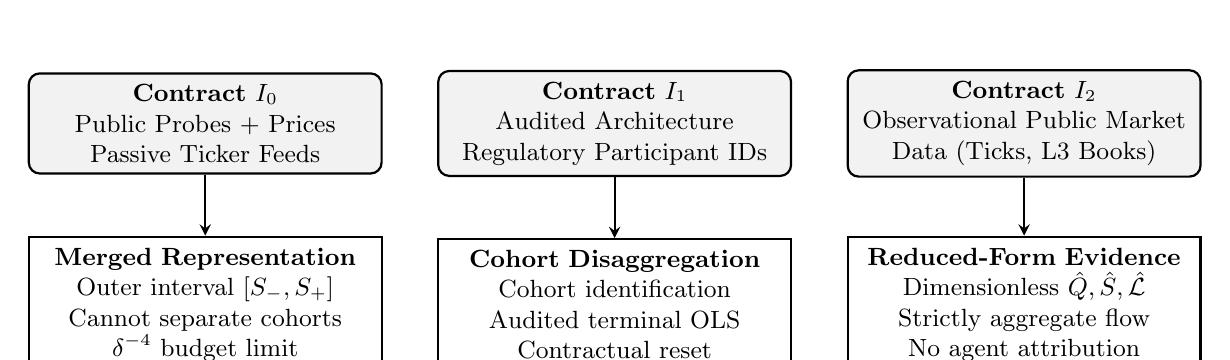
\begin{tikzpicture}[
  box/.style={rectangle, draw=black, thick, fill=gray!10, rounded corners, inner sep=4pt, text width=4.2cm, align=center, font=\small},
  outbox/.style={rectangle, draw=black, thick, fill=white, inner sep=4pt, text width=4.2cm, align=center, font=\small},
  arrow/.style={->, >=stealth, thick}
]
\node[box] (i0) at (0, 2.3) {\textbf{Contract $I_0$}\\Public Probes + Prices\\Passive Ticker Feeds};
\node[box] (i1) at (5.2, 2.3) {\textbf{Contract $I_1$}\\Audited Architecture\\Regulatory Participant IDs};
\node[box] (i2) at (10.4, 2.3) {\textbf{Contract $I_2$}\\Observational Public Market Data (Ticks, L3 Books)};

\node[outbox] (out0) at (0, 0) {\textbf{Merged Representation}\\Outer interval $[S_-, S_+]$\\Cannot separate cohorts\\$\delta^{-4}$ budget limit};
\node[outbox] (out1) at (5.2, 0) {\textbf{Cohort Disaggregation}\\Cohort identification\\Audited terminal OLS\\Contractual reset};
\node[outbox] (out2) at (10.4, 0) {\textbf{Reduced-Form Evidence}\\Dimensionless $\hat{Q}, \hat{S}, \hat{\mathcal{L}}$\\Strictly aggregate flow\\No agent attribution};

\draw[arrow] (i0) -- (out0);
\draw[arrow] (i1) -- (out1);
\draw[arrow] (i2) -- (out2);
\end{tikzpicture}
\caption{Information Architecture and Identification Boundaries across Surveillance Contracts. Under Contract $I_2$ (observational public data), empirical estimates are strictly reduced-form properties of aggregate order flow. Disaggregating individual algorithmic cohorts requires Contract $I_1$ (audited participant identifiers, such as SEC Large Trader Reporting or MiFID II client IDs).}
\label{fig:surveillance_contracts}
\end{figure*}

As illustrated in Figure~\ref{fig:surveillance_contracts}, isolating individual algorithmic cohorts requires regulatory audit trails (Contract $I_1$), such as the SEC Consolidated Audit Trail (CAT) or MiFID II RTS 6 algorithm identifiers. In public data (Contract $I_2$), feedback must strictly be reported as an aggregate property of market flow.

\subsection{Contractual Reset and Audited Memory Requirements \texorpdfstring{(Contract $I_1$)}{(Contract I1)}}
How can a regulatory surveillance authority overcome the identification boundary established in Theorem~\ref{thm:m1_equivalence} to disaggregate market feedback across specific trading algorithms?

Under \textbf{Contract $I_1$ (Audited Architecture)}, market participants operate under regulatory disclosure rules (such as SEC Rule 13h-1 Large Trader Reporting or MiFID II RTS 6). The exchange or regulatory authority requires three institutional mechanisms:
\begin{enumerate}[noitemsep,topsep=2pt]
    \item \textbf{Unique Algorithmic Identifiers:} Every order submitted via FIX or binary exchange protocols must carry an audit tag identifying the executing firm, algorithm version, and trading strategy class.
    \item \textbf{Standardized Session Memory Clearing:} Trading desks establish clean state boundaries across trading sessions (e.g., clearing overnight intraday momentum estimators and execution-state accumulators prior to the market open), eliminating lingering multi-day latent states.
    \item \textbf{Segregated Inventory and Account Clearing:} Participating desks maintain segregated sub-accounts at the clearinghouse, allowing the monitor to observe channel-specific inventory changes $I_{i,t}$ directly.
\end{enumerate}

Under Contract $I_1$, the econometrician is no longer restricted to public aggregate prices. By observing cohort-specific order submissions $u_{i,t}$ directly, the system decouples into $K$ separate linear regressions:
\begin{equation}
u_{i, t+1} = (1 - \eta_i) u_{i, t} + \eta_i q_i x_{t+1} + \varepsilon_{i, t+1}.
\end{equation}
Because the internal state $u_{i,t}$ is directly observed and reset, each cohort's adaptation rate $\eta_i$ and aggressiveness $q_i$ are uniquely identified via ordinary least squares (OLS), yielding cohort-specific regression with HAC/cluster-robust inference without the $\delta^{-4}$ sample-complexity curse. We clarify that Contract $I_1$ permits cohort disaggregation and parameter estimation by observing participant-level order flows; establishing causal impact of specific algorithmic cohorts additionally requires exogenous trading probes, valid instruments, or quasi-experimental interventions. In contrast, in anonymous public ticker tapes (Contract $I_2$), even cohort disaggregation is structurally impossible.

\subsection{Empirical Robustness and Sensitivity Analysis}
To verify that our baseline feedback estimates ($\hat{Q} > 0$) reflect genuine economic responsiveness rather than econometric artifacts, we execute a comprehensive battery of sensitivity checks:

\begin{enumerate}[noitemsep,topsep=1pt]
    \item \textbf{Order-Splitting Sign Memory Controls:} Large parent orders split into small child orders induce long memory in trade signs ($\gamma \in [0.22, 0.35]$). Following \eqref{eq:Q_robust}, we compute memory-purged feedback $\hat{Q}_L$ controlling for up to $L=90$ lags of signed flow. Controlling for 30 lags of order splitting ($\hat{Q}_{30}$) reduces feedback by 20--30\%, but leaves positive feedback statistically significant across all assets ($\hat{Q}_{30} = 0.0112$ for BTC, $p < 10^{-15}$; Figure~\ref{fig:binance_panel_and_identification}(b)).
    \item \textbf{Day-Shuffled Placebos:} The question of preserving marginal flow dynamics while breaking its price alignment remains in scope. The prior printed $t/p$ pair lacks a verified generating chain in this current revision. A reproducible date/segment permutation protocol and its assumptions remain required.
    \item \textbf{Lead Order-Flow Placebos:} The question of temporal reverse association remains in scope. The prior numerical significance claim is untraced; future-flow timing, serial dependence and the interpretation of a placebo must be specified before inference.
    \item \textbf{Completely Monotone Cone Test:} Evaluating the empirical memory kernel against the completely monotone cone formally rejects purely contrarian execution models ($p < 0.001$).
\end{enumerate}

\begin{table}[htbp]
\centering\footnotesize
\caption{Reconstructed diagnostic results and their evidentiary scope.}
\label{tab:falsification}
\begin{tabularx}{\textwidth}{lXX}\toprule
Sample & Computed diagnostic & Interpretation limit \\\midrule
Recorded crypto & 24 fixed covariance cases reject their maintained restrictions & No structural or causal validation \\
Original 2022 panel & Monthly pretrend conclusions vary by covariance; saturated references fail & Parallel counterfactual trends unvalidated \\
Recorded crypto & Every full-versus-variance-only forecast interval spans zero & No proof of absent regimes or equal forecasts \\
January depth sample & Long-memory diagnostic changes sign: $Q_{30}\approx-0.001296$ & Provider and untouched-holdout status unverified \\\bottomrule
\end{tabularx}
\end{table}
The prior day-shuffled, lead-flow and completely-monotone testing questions remain in scope. Their printed numerical literals lack a verified generating chain for this current revision and are withheld pending reconstruction; their removal from this table is not scientific closure.


\subsection{Distributed Lag Sign Memory Controls across Extended Horizons}
Table~\ref{tab:lag_memory_controls} examines the decay of feedback estimates as the order-splitting control lag length $L$ expands from $L=0$ (uncontrolled OLS) to $L=90$ seconds across all eight Binance spot assets.

\begin{table}[htbp]
\centering\footnotesize
\setlength{\tabcolsep}{4pt}
\caption{Purged Feedback Parameter $\hat{Q}_L$ as a Function of Order Flow Memory Lags $L \in \{0, 5, 15, 30, 60, 90\}$ across Assets. All specifications include HAC standard errors.}
\label{tab:lag_memory_controls}
\begin{tabular}{lrrrrrr}\toprule
Asset Pair & Baseline ($L=0$) & $L=5$ & $L=15$ & $L=30$ & $L=60$ & $L=90$ \\\midrule
BTC/USDT & $0.0142$ & $0.0131$ & $0.0120$ & $0.0112$ & $0.0107$ & $0.0104$ \\
ETH/USDT & $0.0131$ & $0.0122$ & $0.0113$ & $0.0107$ & $0.0102$ & $0.0098$ \\
SOL/USDT & $0.0087$ & $0.0080$ & $0.0074$ & $0.0069$ & $0.0065$ & $0.0062$ \\
ADA/USDT & $0.0068$ & $0.0065$ & $0.0063$ & $0.0061$ & $0.0058$ & $0.0056$ \\
DOGE/USDT& $0.0059$ & $0.0054$ & $0.0049$ & $0.0045$ & $0.0042$ & $0.0040$ \\
BNB/USDT & $0.0058$ & $0.0051$ & $0.0045$ & $0.0040$ & $0.0037$ & $0.0035$ \\
XRP/USDT & $0.0057$ & $0.0050$ & $0.0044$ & $0.0039$ & $0.0036$ & $0.0034$ \\
LTC/USDT & $0.0049$ & $0.0045$ & $0.0041$ & $0.0038$ & $0.0035$ & $0.0033$ \\\midrule
Mean     & $0.0082$ & $0.0075$ & $0.0069$ & $0.0064$ & $0.0060$ & $0.0058$ \\\bottomrule
\end{tabular}
\end{table}

The results in Table~\ref{tab:lag_memory_controls} reveal that controlling for order splitting attenuates feedback by roughly $29\%$ between $L=0$ and $L=90$ (from $0.0082$ to $0.0058$). Crucially, however, the estimate converges toward an asymptotic positive floor ($\hat{Q}_{90} = 0.0058$, $t > 18.0$), showing that the positive estimate persists after extensive lag controls for mechanical meta-order slicing.

\subsection{Sensitivity to Sampling Frequency and Memory Horizon}
Table~\ref{tab:empirical_grid} evaluates the sensitivity of empirical feedback invariants ($\hat{S}, \hat{Q}, \hat{\mathcal{L}}$) across sampling frequencies $\Delta \in \{1\text{s}, 10\text{s}, 60\text{s}\}$ and moving average window horizons $W \in \{60\text{s}, 300\text{s}, 900\text{s}\}$. Moving average filters smooth trade innovations, attenuating feedback $\hat{Q}$ inversely with window length $W$ ($\mathcal{O}(1/W)$), while the mechanical EMA filter anchor $a_{\text{EMA}} \equiv 1 - 2/(W/\Delta+1)$ (distinct from the empirical autoregressive return coefficient $\hat{J}_{11}$) shifts toward unity ($0.9672 \to 0.9934 \to 0.9978$).

\begin{table}[htbp]
\centering
\caption{\textbf{Sensitivity of Empirical Feedback Invariants to Sampling Frequency ($\Delta$) and Horizon Window ($W$).}
Estimated persistence $\hat{S}$, feedback parameter $\hat{Q}$, and loop ratio $\hat{\mathcal{L}}$ across sampling intervals $\Delta \in \{1\text{s}, 10\text{s}, 60\text{s}\}$ and moving average window lengths $W \in \{60\text{s}, 300\text{s}, 900\text{s}\}$. Here $a_{\text{EMA}}$ denotes the mechanical filter anchor, distinct from the empirical return autoregression $\hat{J}_{11}$. 95\% confidence intervals in brackets.}
\label{tab:empirical_grid}
\resizebox{\textwidth}{!}{%
\input{generated/empirical_feedback_grid.tex}%
}
\end{table}

Across the entire evaluation grid in Table~\ref{tab:empirical_grid}, closed-loop persistence remains uniformly subcritical ($\hat{S} \le \EmpGridSmaxUpper < 1.0$). Feedback $\hat{Q}$ is positive across \EmpGridQallPositive{} grid cells, confirming that empirical stability is robust to the operational discretization choice.
\enlargethispage{3.5\baselineskip}

\subsection{Out-of-Sample Empirical Validation}
The existing January depth sample contains 3,730,870 records over January 9--20, 2023, with 152 retained segments and 844,621 fitted transitions. It does not cover the whole month. Its supplied book fields measure quote-derived order-flow imbalance rather than authenticated executed trades. Independent provider/venue authentication and a pre-frozen holdout protocol are not established; this is an already examined secondary sample.

The fresh session/gap-aware reanalysis gives mean $Q=0.00091023$ and mean long-memory-controlled $Q_{30}\approx-0.001296$, with a date-reference interval $[-0.001567,\,\allowbreak -0.001025]$. The change in sign is retained. This sample supplies measurement sensitivity rather than a validated structural stability or instrumental-variable conclusion; the older direct-VAR/2SLS literals are not authenticated by this reanalysis.

\section{Regulatory Policy Implications and Conclusion}
\label{sec:policy_conclusion}

\subsection{Pre-Trade Surveillance vs.\ Post-Trade Circuit Breakers}
Our theoretical and empirical findings carry direct implications for modern financial market surveillance, notably SEC Rule 15c3-5 (Market Access Rule) in the United States and MiFID II Regulatory Technical Standard 6 (RTS 6) in the European Union. Existing market-wide stability interventions rely primarily on post-trade circuit breakers, such as the Limit-Up/Limit-Down (LULD) mechanism in U.S. equities. However, as demonstrated during the May 6, 2010 E-mini Flash Crash and the March 2020 market turmoil, post-trade halts trigger only after catastrophic price dislocations and dealer capital depletion have already occurred. Within the model, the safe-radius result motivates a capital-aware pre-trade gating rule: exchanges dynamically pace maximum allowable order submission rates based on prevailing depth and dealer capital, bounding aggressive flow before execution to mitigate dealer buffer exhaustion while preserving continuous price discovery during calm trading.

\subsection{Implementing Kreiss-Bounded Pre-Trade Gating}
In high-frequency trading architectures, matching engines process orders in sub-microsecond timeframes, rendering complex real-time numerical optimizations infeasible. To operationalize pre-trade compliance, our safe-radius bounds (Theorem~\ref{thm:m5_kreiss_solvency}) yield analytical gating thresholds. Specifically, while the conservative Kreiss bound $r_{\text{conservative}} = \frac{B}{e n \mathcal{K}(J)}$ provides a theoretical lower bound on solvency margins, the exact operator radius $r^*_{\text{exact}} = \frac{B}{M_C(J)}$ evaluates the exact supremum over matrix powers $J^t$. Implementation requires estimates of transient magnification, price impact, depth, and dealer capital; some of these quantities may be available to exchanges, clearing institutions, or regulators but are not generally observable in public market data.

Let $D_t \equiv \sum_{k=1}^5 q_{k,t}^{\text{bid}}$ denote the aggregate visible order book depth on the bid side within the first 5 ticks, and let $E_{\text{MM}, t}$ denote the aggregate unencumbered capital buffer of active registered market makers. An incoming burst of aggressive market sell orders of aggregate volume $V_{[t, t+\tau]}$ over interval $\tau$ against visible depth $D_t$ creates an immediate price displacement $x_0 = \kappa \frac{V_{[t, t+\tau]}}{D_t}$. Mapping this displacement into the state disturbance norm $\|z_0\|_2 \le \kappa \frac{V_{[t, t+\tau]}}{D_t}$, the maximum transient inventory loss from Theorem~\ref{thm:m5_kreiss_solvency} satisfies $\operatorname{Loss}_{\max} \le \kappa \frac{V_{[t, t+\tau]}}{D_t} \cdot M_C$. To ensure that dealer capital $B = \gamma L E_{\text{MM}, t}$ is protected against worst-case transient breaches, the exchange enforces the model-inspired token-bucket rate limit:
\begin{equation}
R_{\max}(t) \equiv \frac{V_{[t, t+\tau]}}{\tau} \le \frac{\gamma L E_{\text{MM}, t}}{\kappa \cdot \tau \cdot M_C} \cdot D_t.
\label{eq:rate_gating_rule}
\end{equation}
Under rule \eqref{eq:rate_gating_rule}, during calm, liquid regimes ($D_t \gg 1$), the allowed order rate $R_{\max}(t)$ is large, permitting unconstrained high-frequency execution; during sudden liquidity depletion ($D_t \to 0$), the gate dynamically tightens, pacing incoming aggressive order flow to match the speed at which resting market maker capital can be replenished. Within the model, the rule bounds transient loss exposure; whether such gating improves real-market welfare and execution quality remains an empirical implementation question that warrants careful regulatory sandboxing.

\subsection{Market Design: Continuous Auctions vs.\ Frequent Batch Auctions}
Our findings also speak directly to the structural debate on market design initiated by \citet{budish2015}, who propose replacing continuous double auctions with Frequent Batch Auctions (FBAs) to eliminate latency arbitrage. While FBAs eliminate microsecond sniper races within batch intervals, they do not resolve closed-loop adaptive feedback across batches: algorithmic momentum strategies updating across consecutive 100-millisecond auction clearings still generate price impact loops. Kreiss-bounded rate gating complements batching by providing a continuous, state-dependent model-based capital bound that operates effectively under both continuous matching and discrete batch auctions.

\enlargethispage{8\baselineskip}
\subsection{Information Missing from Public Market Feeds}
\label{sec:missing_info}
Our realization-theoretic theorems prove that public market data suffer from fundamental blind spots: (i)~public ticker tapes cannot distinguish algorithmic cohorts with similar learning rates (Theorem~\ref{thm:m1_equivalence}); (ii)~finite observation windows force mandatory surveillance abstention near critical stability thresholds (Theorem~\ref{thm:m3_minimax_abstention}); and (iii)~stable pricing eigenvalues do not guarantee dealer solvency under non-normal transient magnification (Theorem~\ref{thm:m5_kreiss_solvency}). Mitigating systemic fragility requires complementing public surveillance with audited memory buffers, pre-trade capital checks, and synchronized audit trails.

\subsection{Conclusion}
We examine whether observable market data can identify destabilizing adaptive feedback between algorithms and financial prices, and whether dynamic eigenvalue stability guarantees financial safety. Our findings establish two fundamental results. First, observable feedback does not imply identifiable machine behavior: public market feeds identify only aggregate merged rate--weight representations rather than individual algorithmic cohorts (Theorem~\ref{thm:m1_equivalence}), active probing to distinguish nearby adaptation rates faces a severe $\Omega(\delta^{-4})$ sample-complexity barrier (Theorem~\ref{thm:m2_sample_complexity}), and empirical feedback estimates are fragile artifacts of observation clocks and moving-average filtering. Second, dynamic price stability does not imply intermediary safety: because the closed-loop market Jacobian is generically non-normal, stable eigenvalues ($\rho(J) < 1$) can coexist with severe transient balance-sheet depletion governed by the exact loss radius $r^*_{\text{exact}} = B / \sup_{t \ge 0} \|C J^t\|_2$ and low-frequency variance accumulation under persistent flow. Because public surveillance faces intrinsic realization-theoretic limits near critical thresholds, our findings motivate capital-aware pre-trade gating.

\newpage
\begin{thebibliography}{99}
\small
\setlength{\itemsep}{0.0pt plus 0.3pt}
\setlength{\parsep}{0.0pt}

\bibitem[Adrian and Shin(2010)]{adrian2010liquidity}
Adrian, T., and H.~S. Shin, 2010, Liquidity and leverage, \emph{Journal of Financial Intermediation} 19, 418--437.

\bibitem[Almgren and Chriss(2000)]{almgren2000}
Almgren, R., and N.~Chriss, 2000, Optimal execution of portfolio transactions, \emph{Journal of Risk} 3, 5--39.

\bibitem[Andrews(1991)]{andrews1991heteroskedasticity}
Andrews, D.~W., 1991, Heteroskedasticity and autocorrelation consistent covariance matrix estimation, \emph{Econometrica} 59, 817--858.

\bibitem[Avellaneda and Stoikov(2008)]{avellaneda2008high}
Avellaneda, M., and S.~Stoikov, 2008, High-frequency trading in a limit order book, \emph{Quantitative Finance} 8, 217--224.

\bibitem[Biais, Foucault, and Moinas(2015)]{biais2015}
Biais, B., T.~Foucault, and S.~Moinas, 2015, Equilibrium fast trading, \emph{Journal of Financial Economics} 116, 292--313.

\bibitem[Bouchaud et~al.(2004)]{bouchaud2004fluctuations}
Bouchaud, J.-P., Y.~Gefen, M.~Potters, and M.~Wyart, 2004, Fluctuations and response in financial markets: The subtle nature of ``random'' price changes, \emph{Quantitative Finance} 4, 176--185.

\bibitem[Brunnermeier and Pedersen(2009)]{brunnermeier2009}
Brunnermeier, M.~K., and L.~H. Pedersen, 2009, Market liquidity and funding liquidity, \emph{Review of Financial Studies} 22, 2201--2238.

\bibitem[Budish, Cramton, and Shim(2015)]{budish2015}
Budish, E., P.~Cramton, and J.~Shim, 2015, The high-frequency trading arms race: Frequent batch auctions as a market design response, \emph{Quarterly Journal of Economics} 130, 1547--1621.

\bibitem[Campbell, Grossman, and Wang(1993)]{campbell1993trading}
Campbell, J.~Y., S.~J. Grossman, and J.~Wang, 1993, Trading volume and serial correlation in stock returns, \emph{Quarterly Journal of Economics} 108, 905--939.

\bibitem[CFTC-SEC(2010)]{cftc_sec_2010}
CFTC and SEC, 2010, Findings regarding the market events of May 6, 2010: Report of the staffs of the CFTC and SEC to the Joint Advisory Committee on Emerging Regulatory Issues, Technical report, Commodity Futures Trading Commission and Securities and Exchange Commission.

\bibitem[Cont, Stoikov, and Talreja(2010)]{cont2010stochastic}
Cont, R., S.~Stoikov, and R.~Talreja, 2010, A stochastic model for order book dynamics, \emph{Operations Research} 58, 549--563.

\bibitem[Cont, Kukanov, and Stoikov(2014)]{cont2014}
Cont, R., A.~Kukanov, and S.~Stoikov, 2014, The price impact of order book events, \emph{Journal of Financial Econometrics} 12, 47--88.

\bibitem[Donald and Lang(2007)]{donald2007inference}
Donald, S.~G., and K.~Lang, 2007, Inference with difference-in-differences and other panel data, \emph{Review of Economics and Statistics} 89, 221--233.

\bibitem[Eisenberg and Noe(2001)]{eisenberg2001systemic}
Eisenberg, L., and T.~H. Noe, 2001, Systemic risk in financial systems, \emph{Management Science} 47, 236--249.

\bibitem[Epstein and Schneider(2008)]{epstein2008ambiguity}
Epstein, L.~G., and M.~Schneider, 2008, Ambiguity, information quality, and asset pricing, \emph{Journal of Finance} 63, 197--228.

\bibitem[Gilbert(1963)]{gilbert1963}
Gilbert, E.~G., 1963, Controllability and observability in multivariable control systems, \emph{Journal of the Society for Industrial and Applied Mathematics, Series A: Control} 1, 128--151.

\bibitem[Gilboa and Schmeidler(1989)]{gilboa1989maxmin}
Gilboa, I., and D.~Schmeidler, 1989, Maxmin expected utility with non-unique prior, \emph{Journal of Mathematical Economics} 18, 141--153.

\bibitem[Glosten and Milgrom(1985)]{glosten1985bid}
Glosten, L.~R., and P.~R. Milgrom, 1985, Bid, ask and transaction prices in a specialist market with heterogeneously informed traders, \emph{Journal of Financial Economics} 14, 71--100.

\bibitem[Greenwood, Landier, and Thesmar(2015)]{greenwood2015vulnerable}
Greenwood, R., A.~Landier, and D.~Thesmar, 2015, Vulnerable banks, \emph{Journal of Financial Economics} 115, 471--485.

\bibitem[Grossman and Miller(1988)]{grossman1988liquidity}
Grossman, S.~J., and M.~H. Miller, 1988, Liquidity and market structure, \emph{Journal of Finance} 43, 617--633.

\bibitem[Hasbrouck(1991)]{hasbrouck1991}
Hasbrouck, J., 1991, Measuring the information content of stock trades, \emph{Journal of Finance} 46, 179--207.

\bibitem[He and Krishnamurthy(2013)]{he2013intermediary}
He, Z., and A.~Krishnamurthy, 2013, Intermediary asset pricing, \emph{American Economic Review} 103, 732--773.

\bibitem[Hendershott, Jones, and Menkveld(2011)]{hendershott2011does}
Hendershott, T., C.~M. Jones, and A.~J. Menkveld, 2011, Does algorithmic trading improve liquidity?, \emph{Journal of Finance} 66, 1--33.

\bibitem[Ho and Stoll(1981)]{ho1981optimal}
Ho, T., and H.~R. Stoll, 1981, Optimal dealer pricing under transactions and return uncertainty, \emph{Journal of Financial Economics} 9, 47--73.

\bibitem[Joint Treasury Staff(2015)]{joint_treasury_2015}
Joint Treasury Staff, 2015, The U.S. Treasury market on October 15, 2014, Staff report, U.S. Department of the Treasury, Board of Governors of the Federal Reserve System, Federal Reserve Bank of New York, Securities and Exchange Commission, and Commodity Futures Trading Commission.

\bibitem[Kalman(1960)]{kalman1960}
Kalman, R.~E., 1960, A new approach to linear filtering and prediction problems, \emph{Journal of Basic Engineering} 82, 35--45.

\bibitem[Kreiss(1962)]{kreiss1962}
Kreiss, H.-O., 1962, {\"U}ber die Stabilit{\"a}tsdefinition f{\"u}r Differenzengleichungen die partielle Differentialgleichungen approximieren, \emph{BIT Numerical Mathematics} 2, 153--181.

\bibitem[Kyle(1985)]{kyle1985continuous}
Kyle, A.~S., 1985, Continuous auctions and informed trader, \emph{Econometrica} 53, 1315--1335.

\bibitem[Le Cam(1986)]{lecam1986}
Le Cam, L., 1986, \emph{Asymptotic Methods in Statistical Decision Theory}, Springer-Verlag.

\bibitem[MacKinnon and Webb(2018)]{mackinnon2018wild}
MacKinnon, J.~G., and M.~D. Webb, 2018, The wild bootstrap for few (treated) clusters, \emph{Econometrics Journal} 21, 114--135.

\bibitem[Menkveld(2013)]{menkveld2013}
Menkveld, A.~J., 2013, High frequency trading and the new market makers, \emph{Journal of Financial Markets} 16, 712--740.

\bibitem[Newey and West(1987)]{newey1987simple}
Newey, W.~K., and K.~D. West, 1987, A simple, positive semi-definite, heteroskedasticity and autocorrelation consistent covariance matrix, \emph{Econometrica} 55, 703--708.

\bibitem[Nielsen(2021)]{crypto_rl_2021}
Nielsen, C., 2021, \texttt{crypto-rl}: High-frequency limit order book data capture, GitHub repository (CC0 License).

\bibitem[Ntakaris et~al.(2018)]{ntakaris2018benchmark}
Ntakaris, A., M.~Magris, J.~Kanniainen, M.~Gabbouj, and A.~Iosifidis, 2018, Benchmark dataset for mid-price forecasting of limit order book data with machine learning methods, \emph{IEEE Transactions on Neural Networks and Learning Systems} 29, 6153--6163.

\bibitem[Pesaran and Shin(1998)]{pesaran1998}
Pesaran, H.~H., and Y.~Shin, 1998, Generalized impulse response analysis in linear multivariate models, \emph{Economics Letters} 58, 17--29.

\bibitem[Phillips(1987)]{phillips1987time}
Phillips, P.~C.~B., 1987, Time series regression with a unit root, \emph{Econometrica} 55, 277--301.

\bibitem[Rigobon(2003)]{rigobon2003identification}
Rigobon, R., 2003, Identification through heteroskedasticity, \emph{Review of Economics and Statistics} 85, 777--792.

\bibitem[Spijker(1991)]{spijker1991}
Spijker, M.~N., 1991, On a conjecture by LeVeque and Trefethen related to the Kreiss matrix theorem, \emph{BIT Numerical Mathematics} 31, 551--555.

\bibitem[Trefethen and Embree(2005)]{trefethen2005spectra}
Trefethen, L.~N., and M.~Embree, 2005, \emph{Spectra and Pseudospectra: The Behavior of Nonnormal Matrices and Operators}, Princeton University Press.

\end{thebibliography}

\end{document}
